\noindent\enquote{\itshape You can never know everything, and part of what you know is always wrong. Perhaps even the most important part. A portion of wisdom lies in knowing that. A portion of courage lies in going on anyways.}\bigbreak

\hfill Lan Mandragoran - Winter's Heart

\vspace*{0.05\textheight}

In this chapter, we introduce a small subset of our previously presented structures to an interacting environment. At the classical level we present the results of a parametric implicit solvation model to qualitatively discuss the effects that an environment may have on the stability and dynamics of structures discussed earlier in Chapter \ref{c:Coal}. These computations will be presented in parallel to a modified form of the Greens Dyadic Method in which the environment is considered to be water. Finally, we briefly present \textit{ab initio} calculations of electrostatics and dynamics of small AuPt nanoalloys interacting with explicit water molecules.

\section{AuPt in an implicit solvation}
\label{Class_Water}

\subsection{Implicit solvation model}

Finally, we characterise the stability of fixed size AuPt nanoalloys with varied chemical ordering and abundance of the two species. For the sake of simplicity, we have limited the configuration space to the core-shell configuration, a Janus type nanostructure, and a random mixing of the two species. In this, we too have varied the abundance whereby in the former instance we have considered various thicknesses of Pt shell enclosing the Au core within. Given that we have fixed the size at 309 atoms, this permits the existence of four complete atomic shells - the core atom notwithstanding. As for the latter two configurations, we have created the Janus in a crude fashion by specifying the desired abundance and setting the chemical species on one side of a dividing line to Au, and on the opposing side to Pt where the dividing line is generated from the specified abundance. As for the random configuration, we have simply generated random numbers from a uniform distribution on the unit interval. Should a value be less than the prescribed abundance, the atom undergoes a forced specie reassignment.

We have elected to use a simplified implicit environment which requires only two parameters to set for each specie present: the interaction energy and the relative strength of the interaction where the former may be set to be a fraction of the specie's cohesive energy and the latter is an exponent whose units are dimensionless. Whilst this model is indeed simplistic, the optimistic perspective is that it provides a broad phase space in which one may search for a qualitatively appropriate parameter set to describe the environment in which a model system may be considered to reside.

Whilst it is true that various solvation models exist \textit{a-priori}, the literature regarding metal-environment interactions with the SMATB potentials described in Table \ref{tab:RGL} is sparse. Given that it is a highly no-trivial problem to tune parameters from an existing solvation model to inter-atomic potentials which are otherwise unsupported, we maintain that it is appropriate to construct a potential set given our prescribed parameterisation so as to exercise a finder degree of control over how the model may interact with our metallic species. Consequently, the purpose of this investigation is to determine if such a model may be appropriate and fit for purpose given the SMATB potentials we have used.

The account of the metal-environment interactions relies on a mean field approach, in which the atoms/molecules of the environment are not explicitly represented (Fig. 1). They are assumed to be homogeneously distributed, without concentration gradients induced by specific attraction or repulsion between them. They provide a coordination dependent energy term to the metal atoms of the form

\begin{equation}
    E_{i,M}^{Env} = -\varepsilon_{M} \left( 12 -  CN_{i} \right) ^{\rho_{M}}
    \label{eqn:env_Lodis}
\end{equation}

We describe in Equation \ref{eqn:env_Lodis} the formulation of the environmental model introduced in \cite{doi:10.1063/1.4811670} where $E_{i}^{Env}$ is the potential energy interaction between atom $i$ and the environment, $\varepsilon_{M}$ is the energy of the interaction itself which may be intuited from the cohesive energy of the given species as detailed in the reference article, and $\rho_{M}$ is the interaction type of the metal. Where one may loosely intuit values of this exponent less than 1 to imply a weak covalent like interaction; equal to 1 is intuitively a pairwise interaction and greater than 1 is strongly interacting. As seen in earlier Chapters, $CN_{i}$ is simply the coordination number of the given atom. 

The metal-environment interaction relies on an additional many~-~body potential which affects surface atoms as a function of their coordination. In this respect, the method is in line with previous studies of MNPs on an oxide substrate \cite{PhysRevB.65.245411,10.1063/1.3077300,PhysRevB.79.165438,PhysRevB.81.155443}. Indeed, that the absolute value of Equation \ref{eqn:env_Lodis} grows reflects the well-established increased reactivity of low-coordinated atoms. Moreover, bulk~-~like atoms are assumed to be inert with respect to the environment, rather feeling its influence implicitly via the surface atoms above.

As discussed in these chapters, it is generally accepted that the number of nearest neighbours a given atom will have in the bulk phase of an FCC environment will be 12, however this may not necessarily be the case. Indeed, as acknowledged in Chapter \ref{c:Theory}, there exist morphologies such as Frank-Kasper polyhedra \cite{https://doi.org/10.1107/S0365110X59001499} which are known to have coordination number as high as 14 \cite{Shoemaker:a25444,NELSON19891,doi:10.1073/pnas.1809655115}. Nonetheless, any atoms who are not present at the surface or exposed to it will not directly feel the interaction - making it highly efficient as one need only compute the list of surface atoms from geometric arguments to truncate the number of potential energy calculations to perform by a factor which scales with the system size. Moreover, the authors of this model report success with respect to experimental observations when considering surface energies, further establishing this model as a viable candidate for the introduction of an environment to NAs acting under SMATB inter~-~atomic potentials.

Whilst it is true that there may exist environment~-~metal pairings with strong long~-~range interactions \cite{doi:10.1021/jp0609941}, it is not uncommon within the context of describing catalytic reactions to consider only the surface~-~solvent/environment interaction and neglect contributions from deeper lying atoms \cite{Rossi2020}. Therefore, despite not necessarily being truly physical, this model and approach is consistent with the methodologies of the SMATB and the catalytic communities.

\begin{figure}[h!]
    \centering
    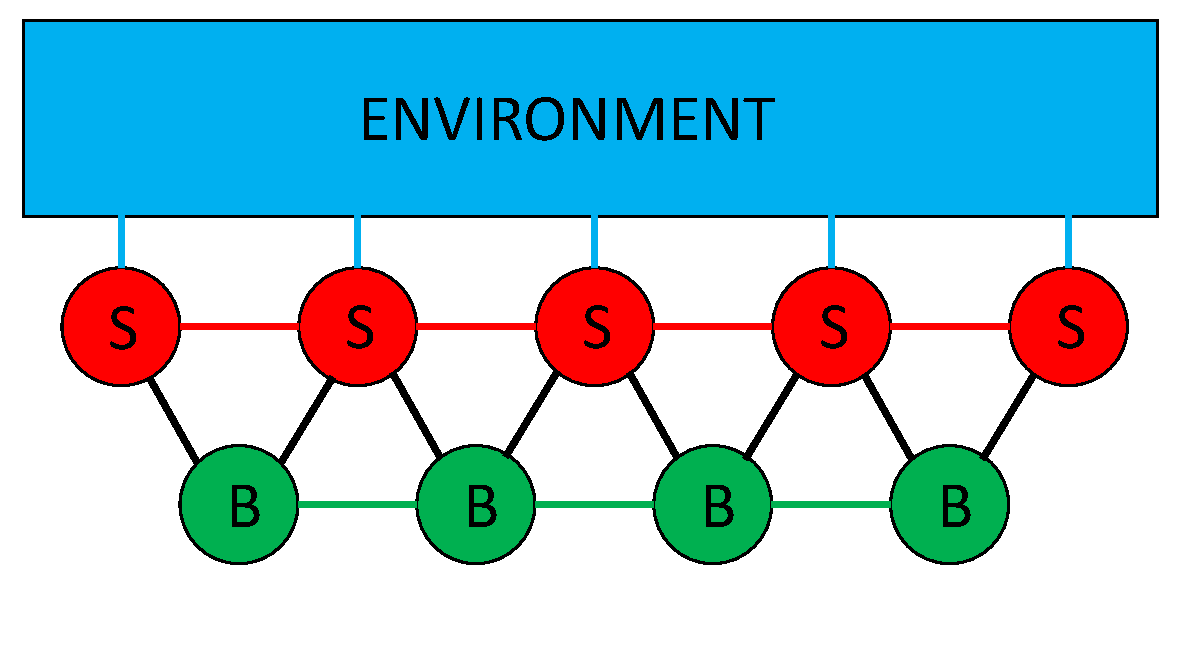
\includegraphics[width=0.95\textwidth]{figures/MD/Env/SMATB_Env.pdf}
    \caption{Schematic diagram of the implicit environment model with interactions implied by sticks, atoms described by balls, and the environment as a sea coupling to the surface atoms. Surface atoms are denoted by the letter `S', bulk atoms are denoted by the letter `B'.}
    \label{fig:SMATB_Env}
\end{figure}

In Figure \ref{fig:SMATB_Env}, an interaction diagram is provided to demonstrate the nature of the model as it is described above. In which the external environment interacts with the NA only via the low coordination surface atoms. Who themselves interact with their neighbours via the SMATB potentials described in Section \ref{sec:CMD}.

To perform  simulations with our parameters, ensuring that our results may be sensible when we perform further computations, we first considered the case of monometallic Au and Pt separately, so as to see how in the isolated case these metals may respond to the interaction of the environment.

\begin{figure}[h!]
     \centering
         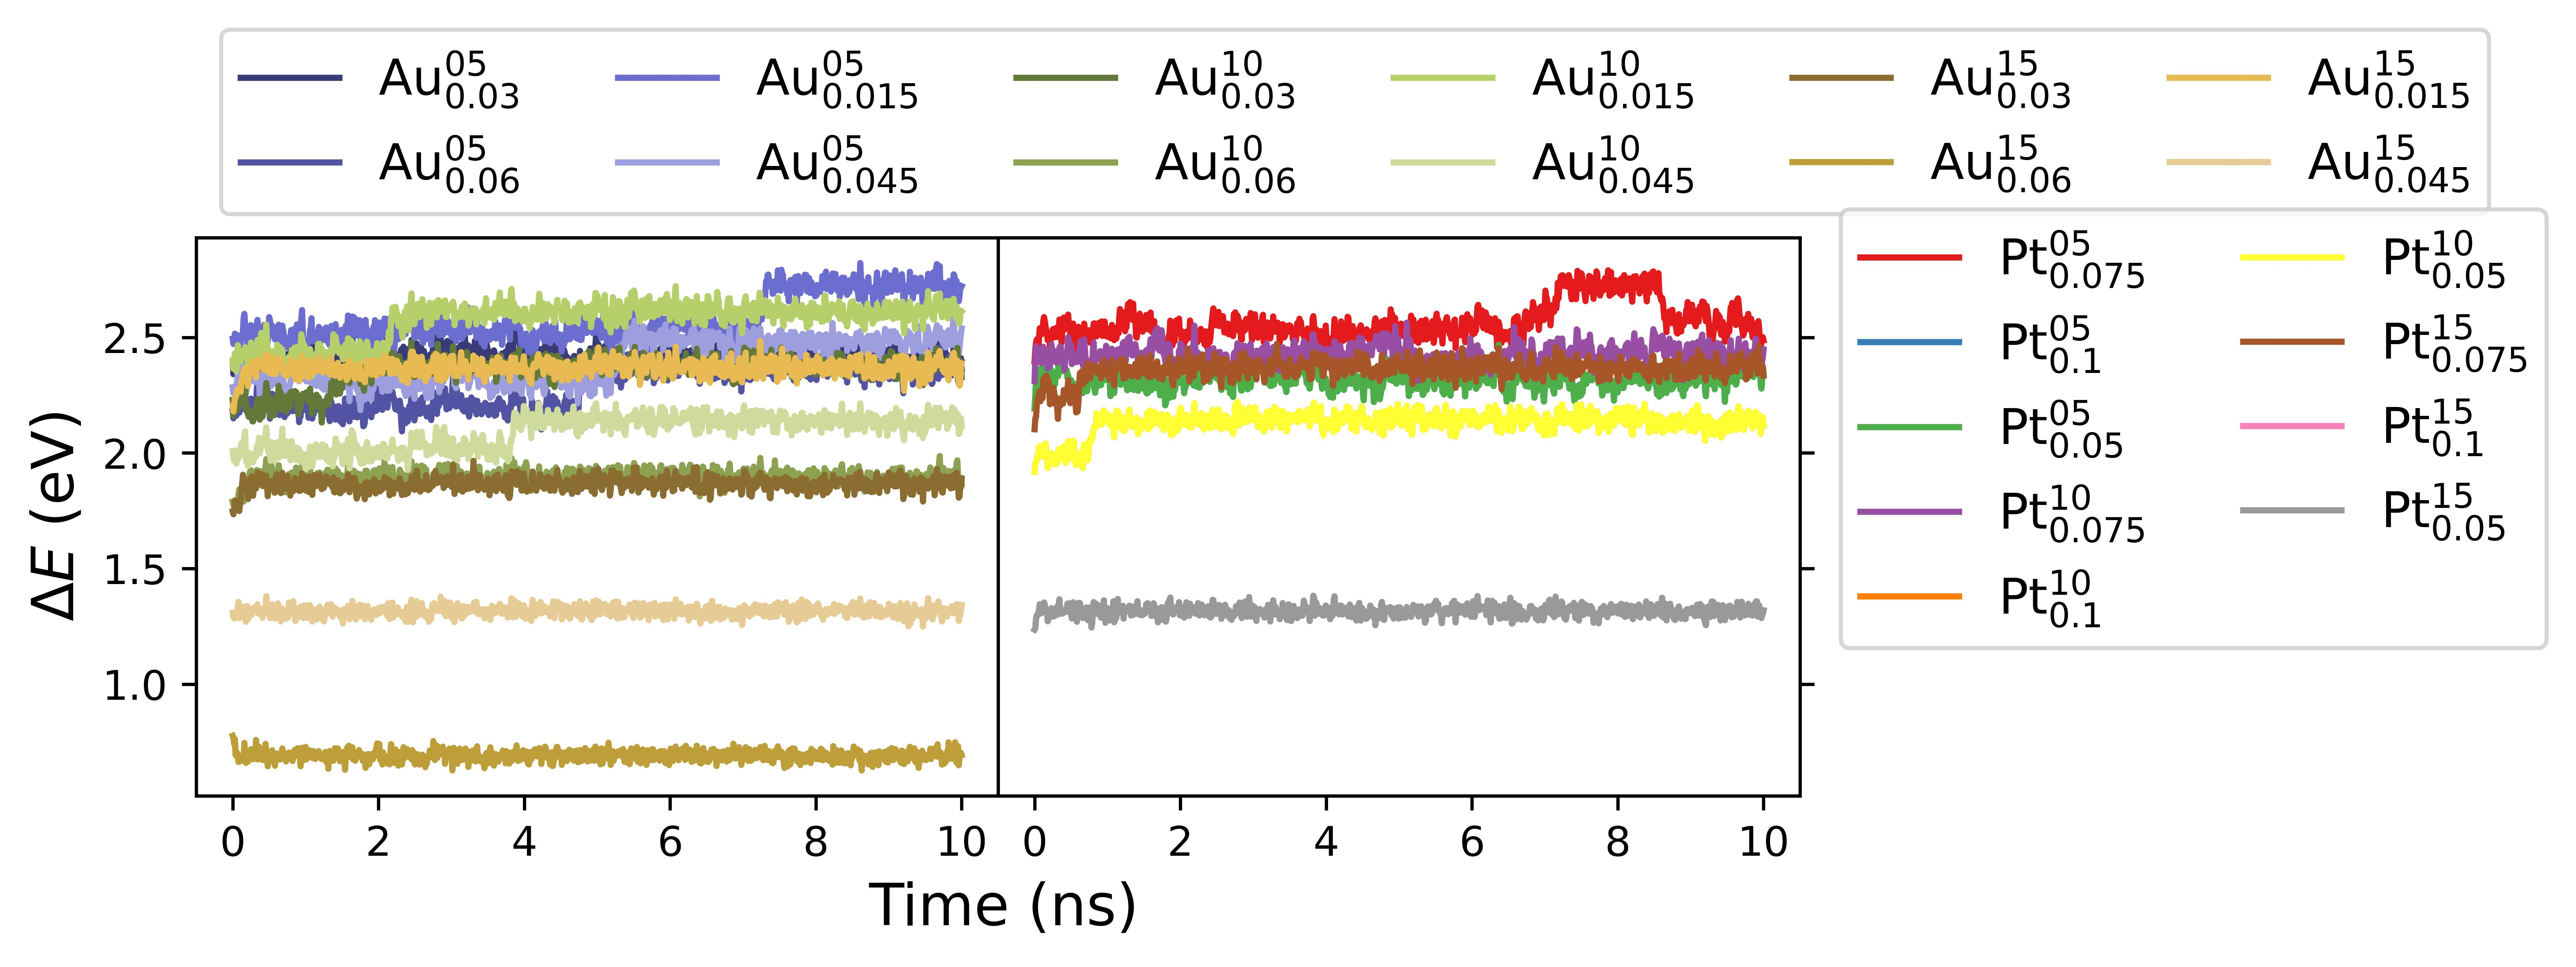
\includegraphics[width=0.95\textwidth]{figures/MD/Env/Env_Pure.jpeg}
    \caption{Excess energy varying the $\eta_{Au}$ and $\eta_{Pt}$ for pure metallic systems. Left panel describes the pure Au$_{309}^{Ih}$ cluster. Right is the Pt$_{309}^{Ih}$ cluster. All simulations run for 10 ns at 600 K under NVT conditions.}
    \label{fig:Pure_eta}
\end{figure}

In Figure \ref{fig:Pure_eta}, we report the excess energy of the cluster, defined in Equation \ref{eqn:excessE}, as a function of time across a brief molecular dynamics simulation for each of the permutations of $\varepsilon$ and $\rho$ for each given metal. Already, we note the profound influence that the introduction of an environment has on the bare clusters alone. As our intuition would suggest, a strongly coupled environment with a small interaction energy will result in a more stable configuration with lower potential energy. The former is trivially true, in that a strongly coupled environment will favour a structure that minimises their surface to volume ratio - \textit{i.e.,} a sphere - whereby the Ih morphology is the most spherical in morphology whilst maintaining its structural integrity. As for the latter assertion, to verify this we must reconsider Equation \ref{eqn:excessE} and recall that the only parameter we change is indeed the total energy. Consequently a larger total energy, which is causally related to the potential energy arising from the environment, will manifest as a higher $\Delta E$.

When now considering the converse, in the weakly interacting regime, we we observe fluctuations in the $\Delta E$ quantity which is typically an indicator for structural rearrangement \cite{LaiaMelt}. Whilst the background temperature is too low for melting to occur, it is still sufficiently thermally active for surface atoms to become mobile and for the core of the structure to become disordered.

\subsection{Energetic evolution}

\begin{figure}
\centering
\begin{subfigure}[b]{0.8\textwidth}
    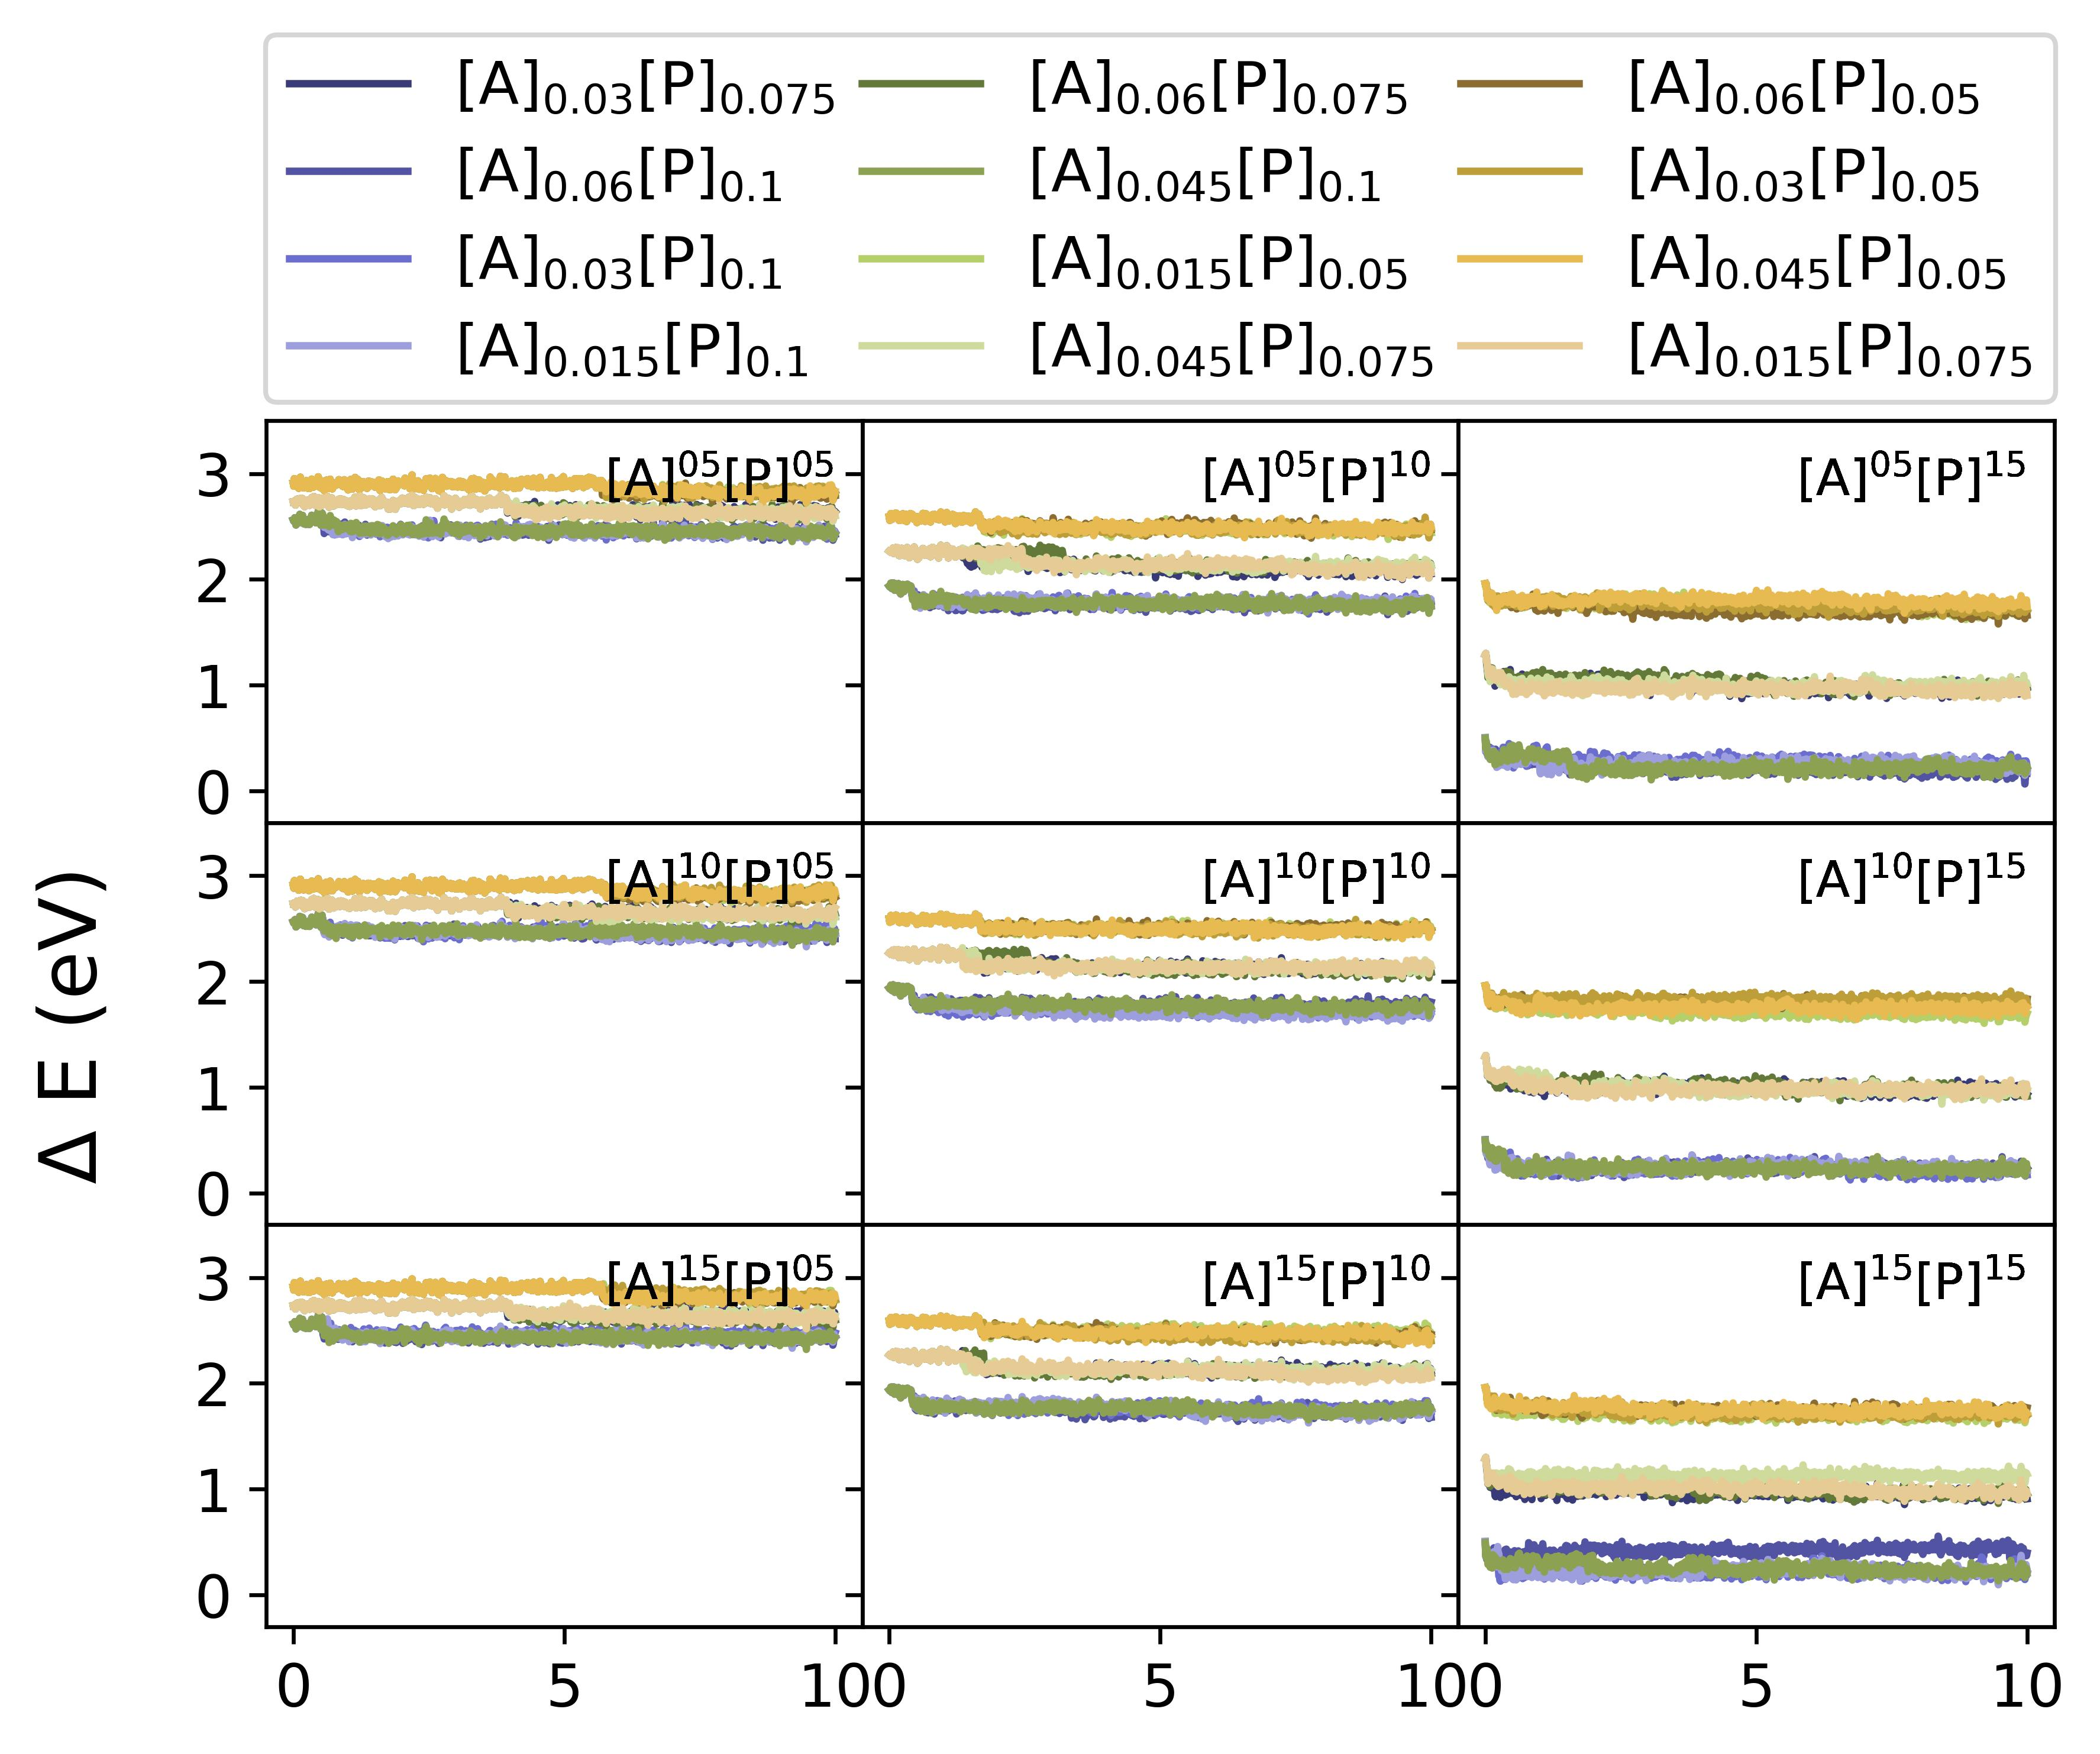
\includegraphics[width=\textwidth]{figures/MD/Env/CS1_EDelta.jpeg}
\end{subfigure}\\
\begin{subfigure}[b]{0.8\textwidth}
    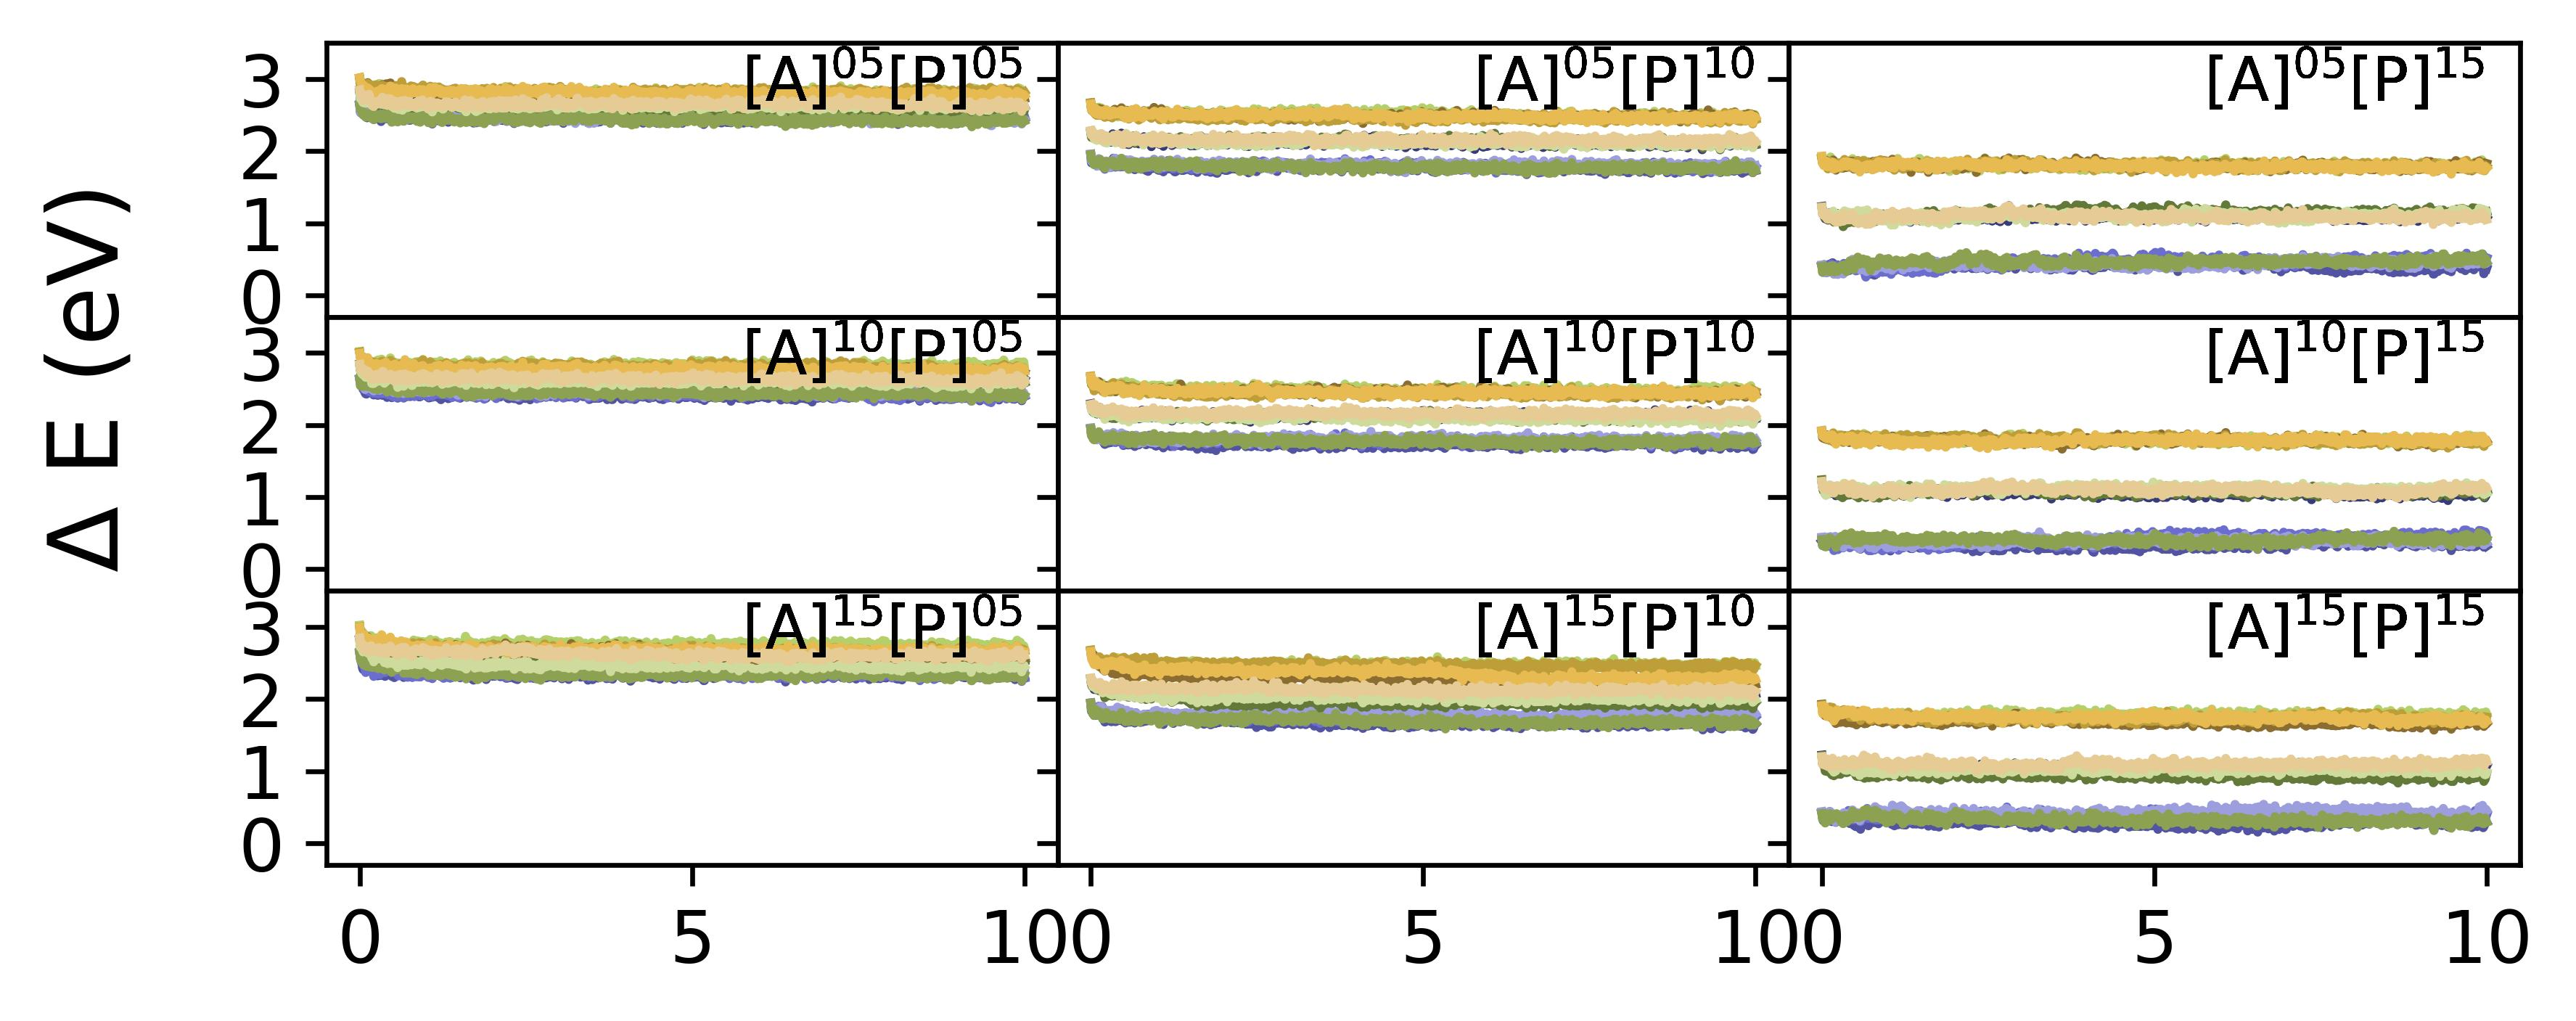
\includegraphics[width=\textwidth]{figures/MD/Env/CS2_EDelta.jpeg}
    \end{subfigure}\\
\begin{subfigure}[b]{0.8\textwidth}
    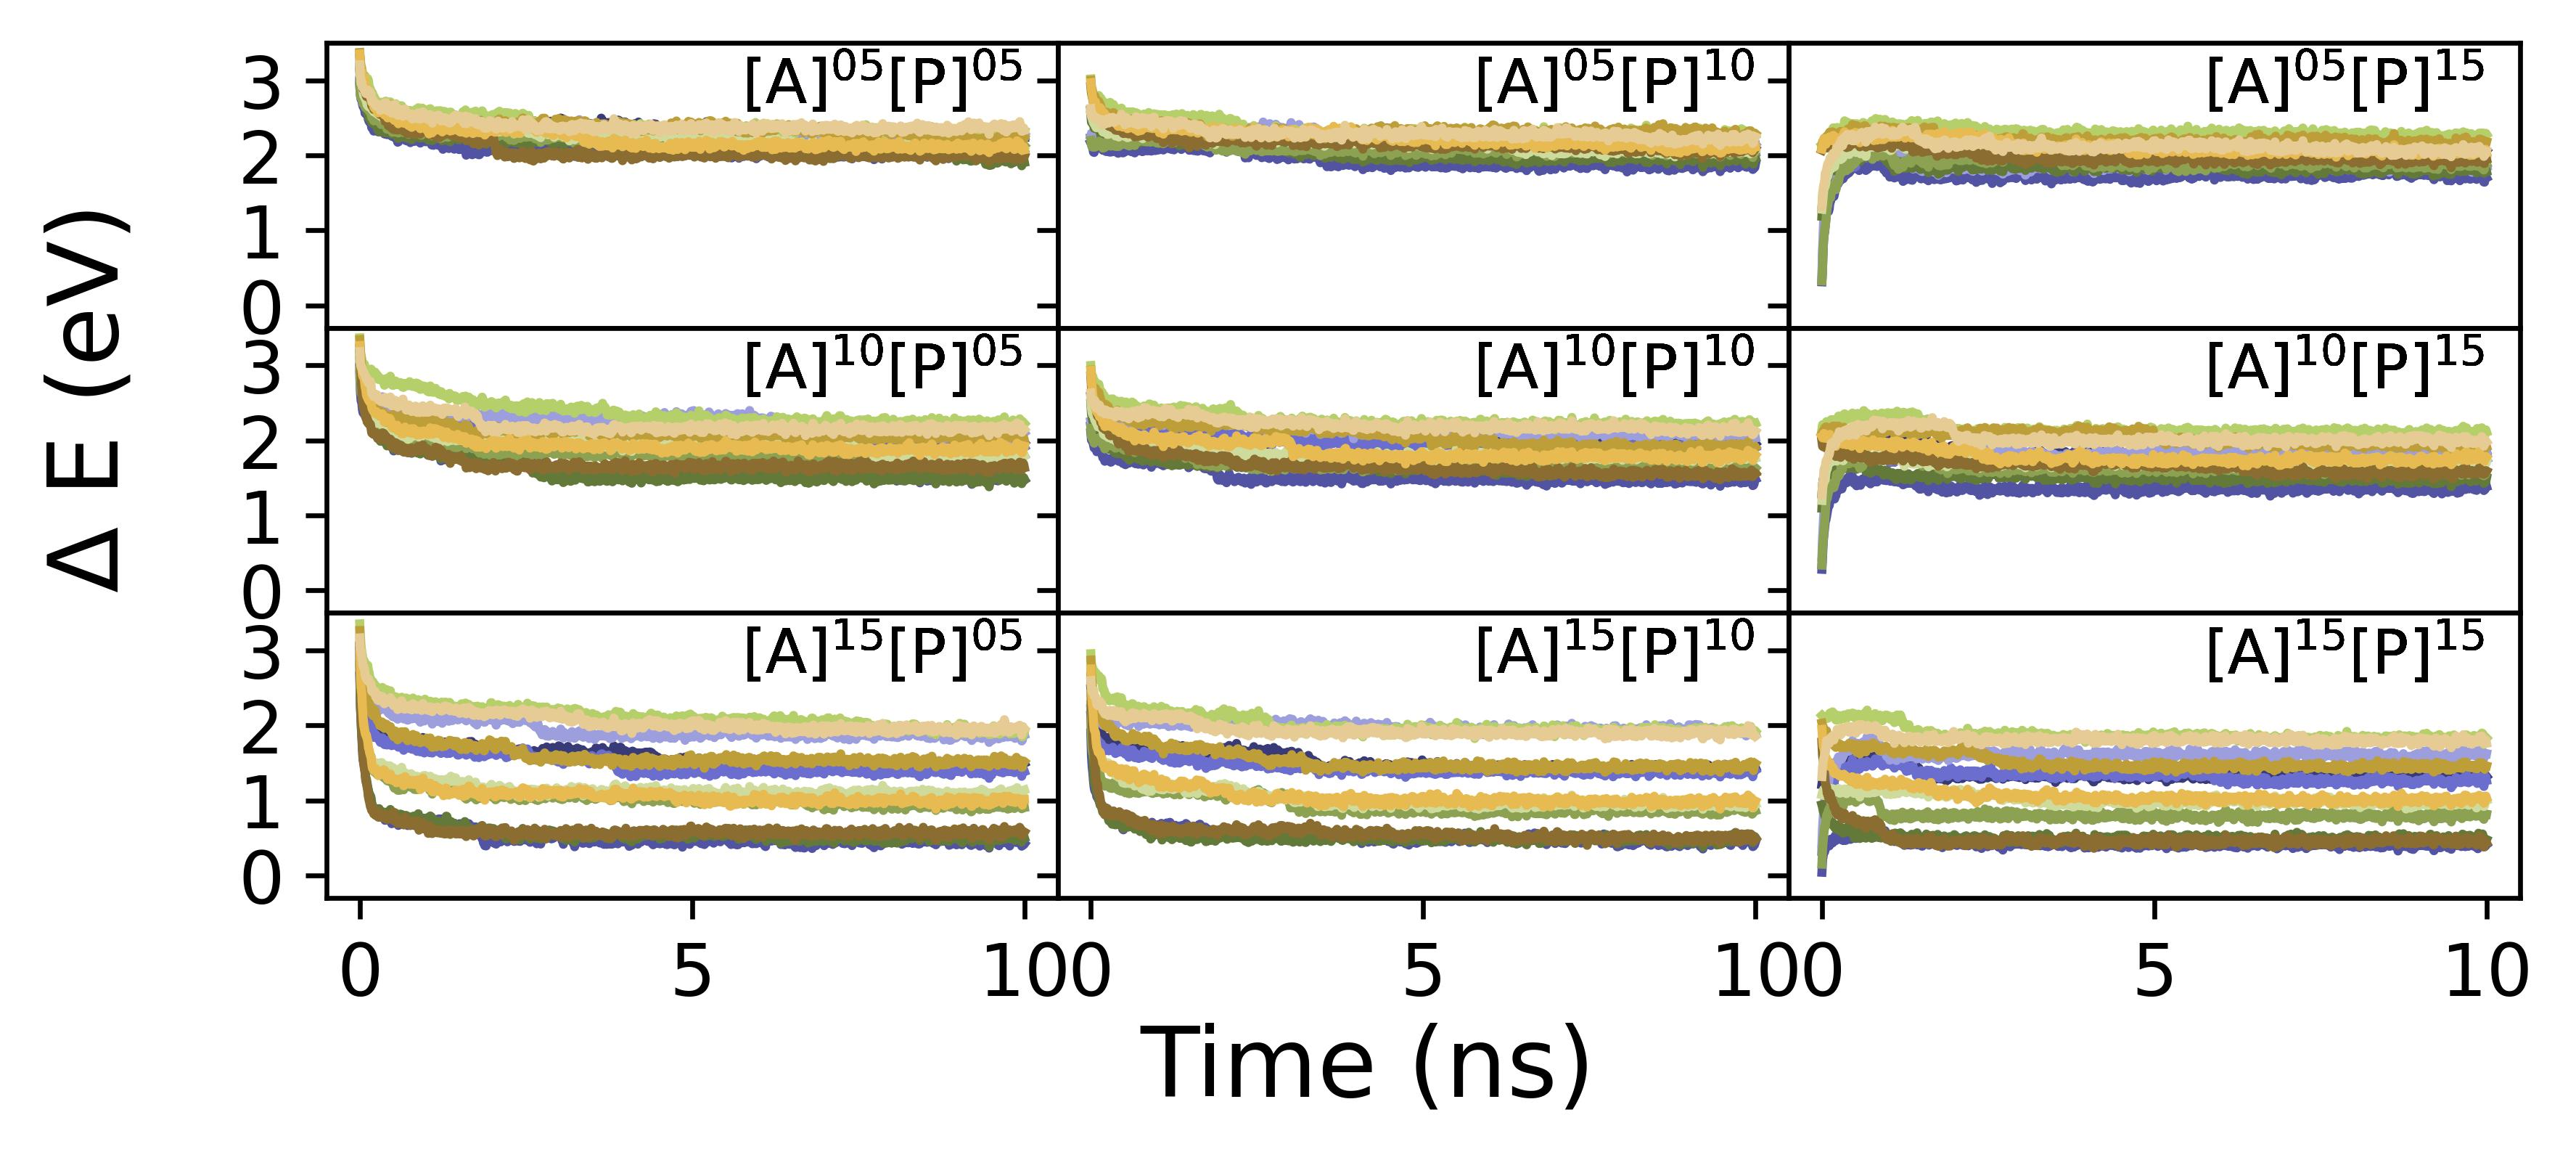
\includegraphics[width=\textwidth]{figures/MD/Env/CS3_EDelta.jpeg}
\end{subfigure}
    \caption{$\Delta E$ plotted versus time for the various environment parameters tested on the core-shell chemical ordering. Each sub-figure presents all time series for a given specified morphology and shares common line colour schemes and axes. Each block is for the given $\rho_{Au}\rho_{Pt}$ parameters, and each line represents a pair of $\varepsilon_{Au}\varepsilon_{Pt}$ coupling strengths. The top three panels are for the Au$_{13}^{Ih}$Pt$_{296}^{Shell}$. The next three panels are Au$_{55}^{Ih}$Pt$_{254}^{Shell}$. The final three are Au$_{147}^{Ih}$Pt$_{162}^{Shell}$. }
    \label{fig:Delta_E_Env_CS}
\end{figure}

In Figure \ref{fig:Delta_E_Env_CS} we present the evolution of the excess energy with respect to time for the Core-Shell AuPt structures where we have varied the shell thickness in addition to the solvent model parameters. In general, we may assert that when the Au-solvent interaction is stronger or equal to that of Pt-solvent and there is an appreciable amount of Au at the centre, there is a clear indication that the structure is able to undergo some form of atomic reconfiguration as displayed by the drop in the value of $\Delta E$ which is commonly observed when the total energy of the cluster tends towards the total energy. As we discussed in the previous chapter, it is typically the strongly cohesive nature of Pt which allows the nanoalloy to resist large scale restructuring and frustrates the effort to move towards a more energetically favourable configuration. Here we see precisely this when there exists a monolayer of Pt covering the Au core, seen in the bottom set of panels of Figure \ref{fig:Delta_E_Env_CS}. Otherwise, it appears that there is no significant evolution in $\Delta E$ when there is a large volume of Pt covering the inner Au core. 

\begin{figure}
\centering
\begin{subfigure}[b]{0.8\textwidth}
    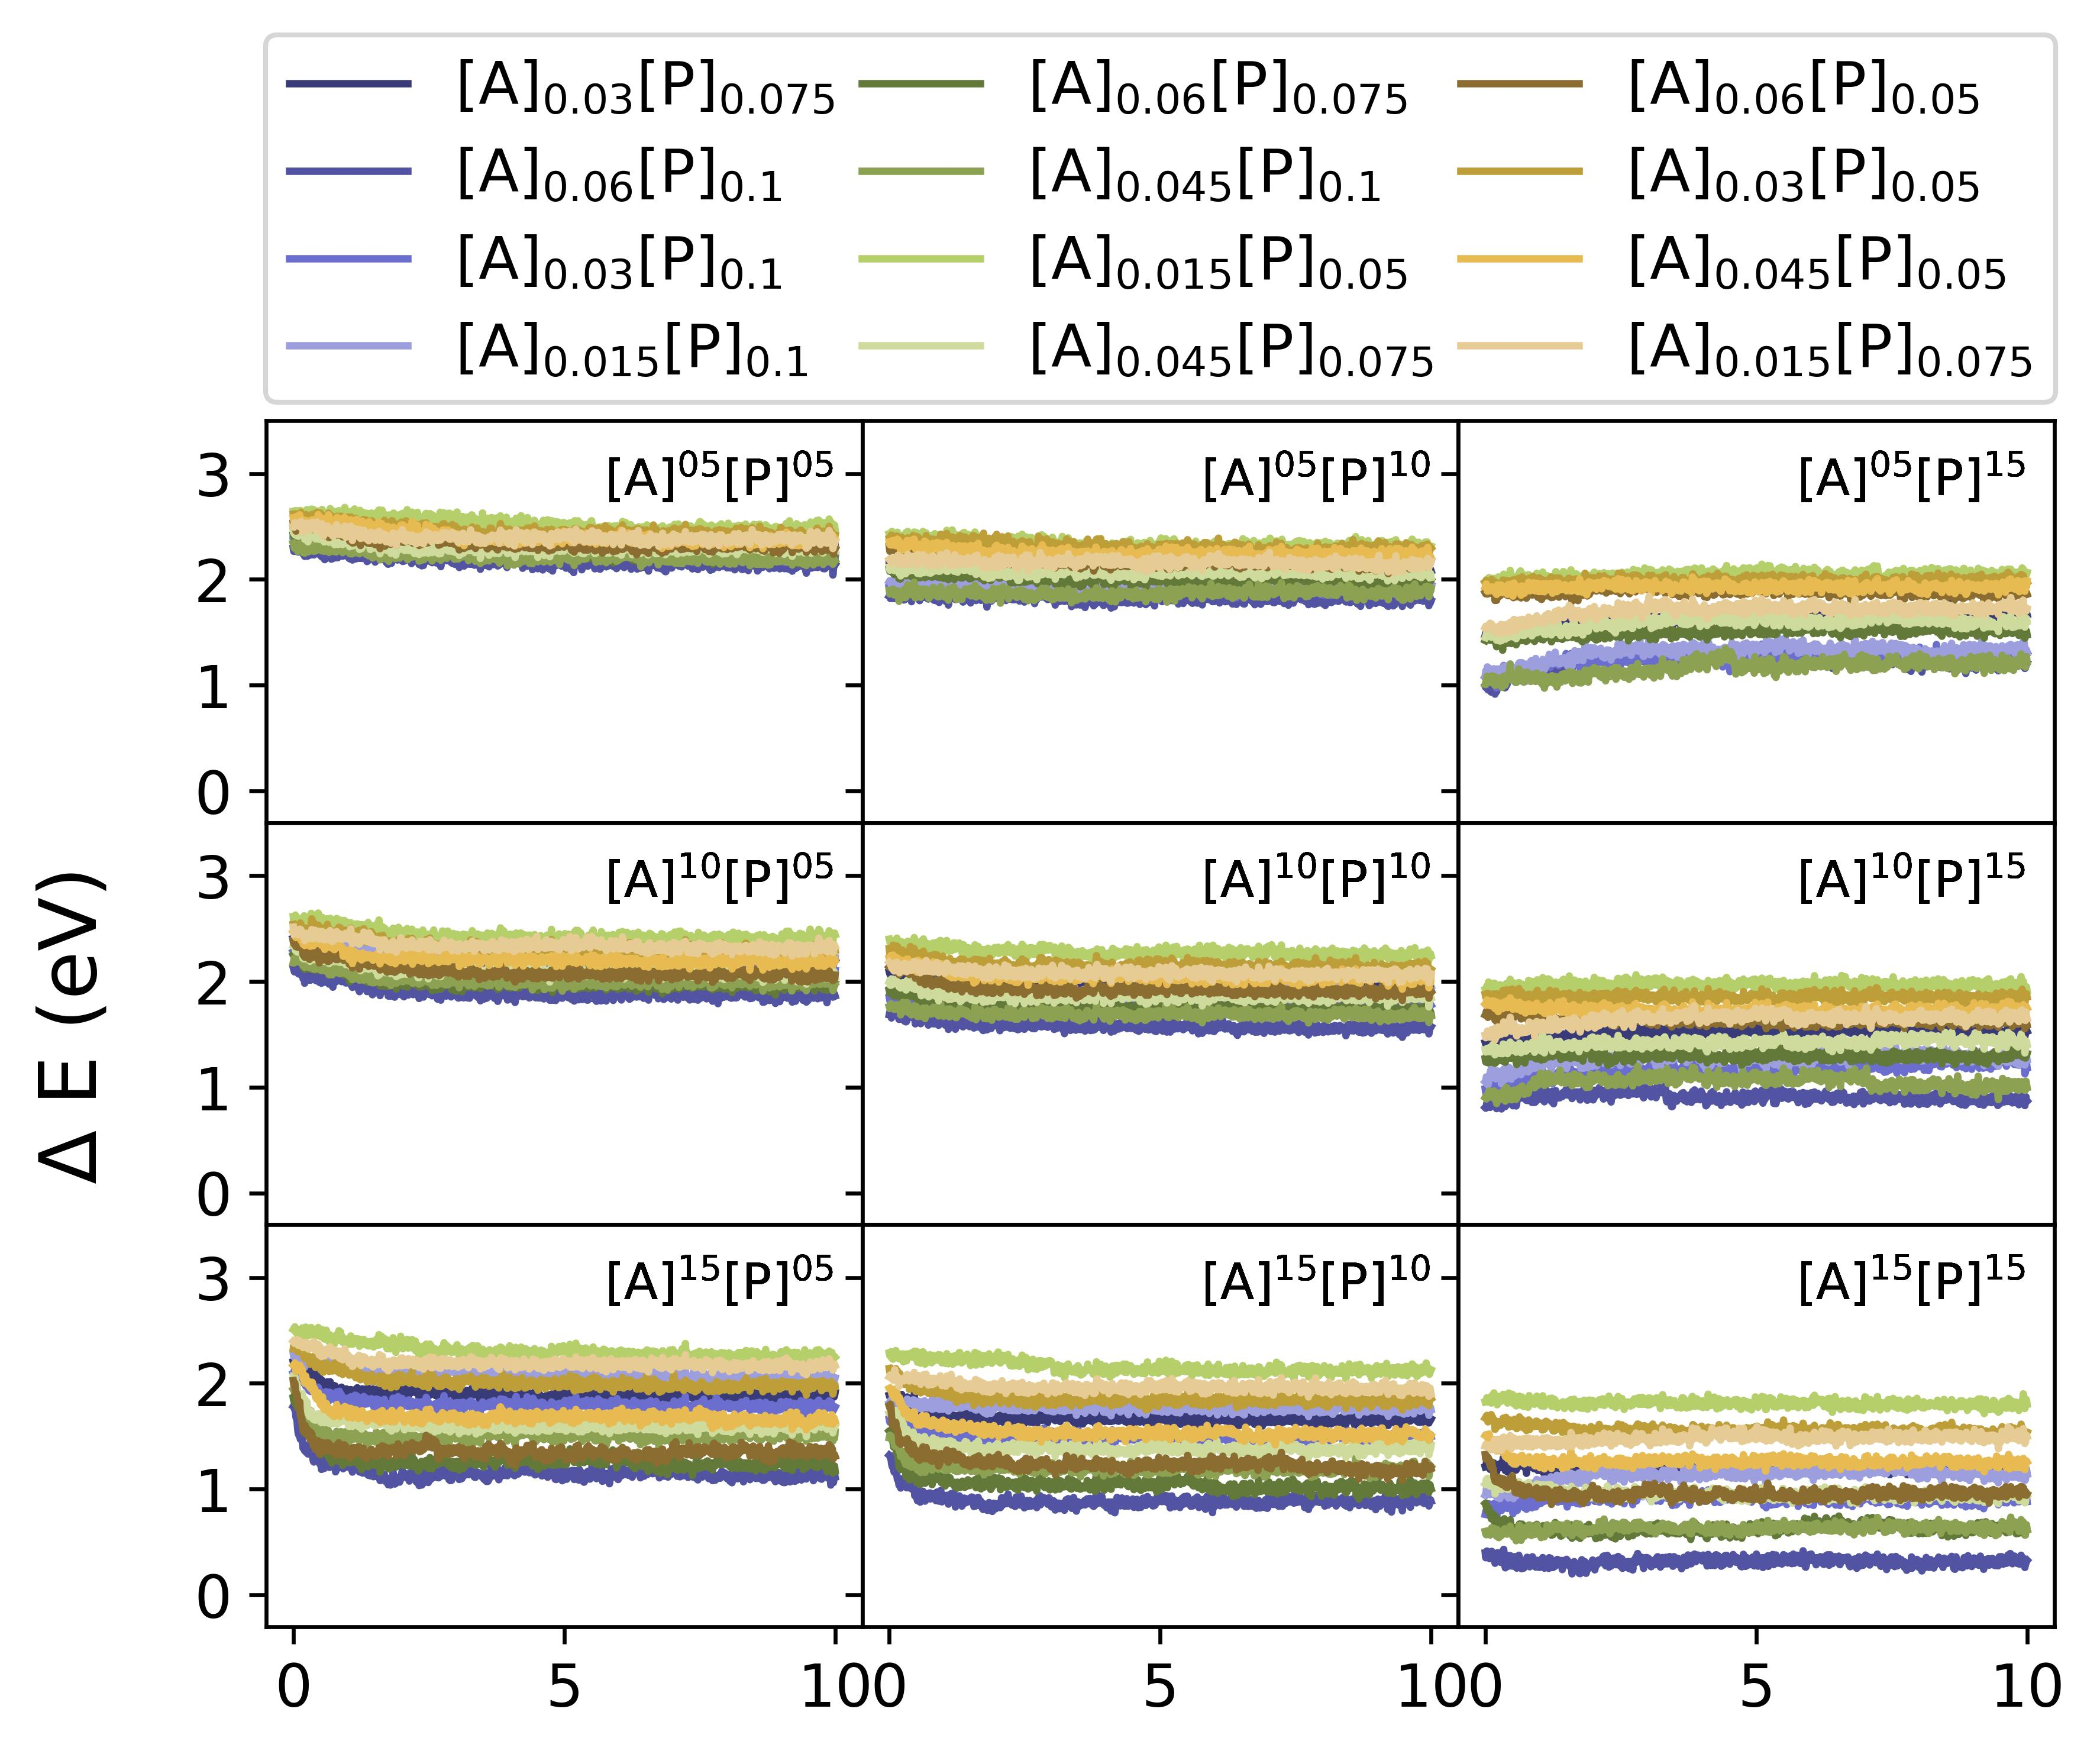
\includegraphics[width=\textwidth]{figures/MD/Env/Jan25_EDelta.jpeg}
\end{subfigure}\\
\begin{subfigure}[b]{0.8\textwidth}
    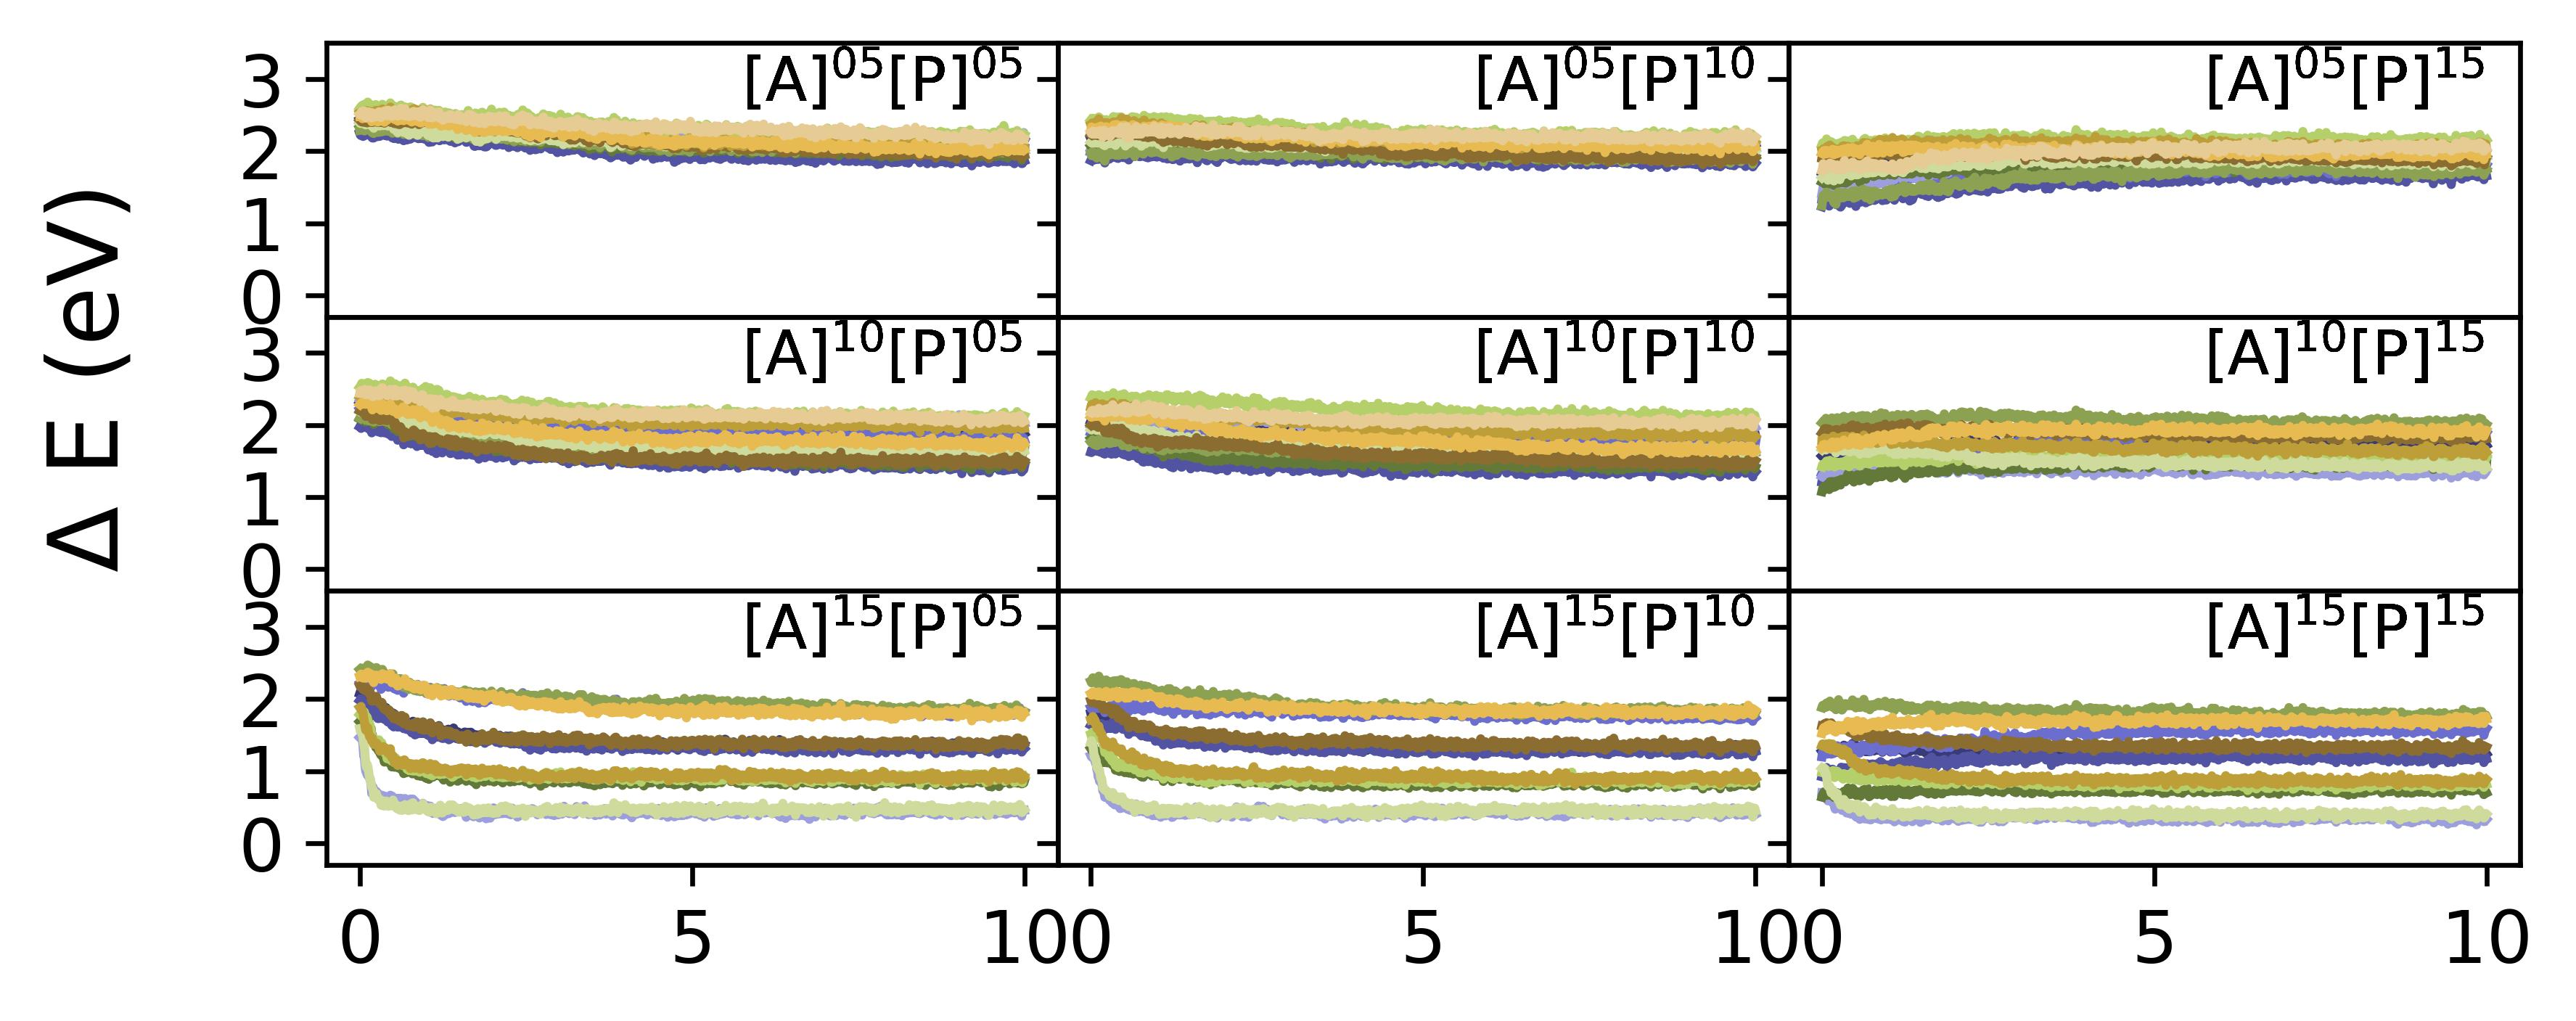
\includegraphics[width=\textwidth]{figures/MD/Env/Jan50_EDelta.jpeg}
    \end{subfigure}\\
\begin{subfigure}[b]{0.8\textwidth}
    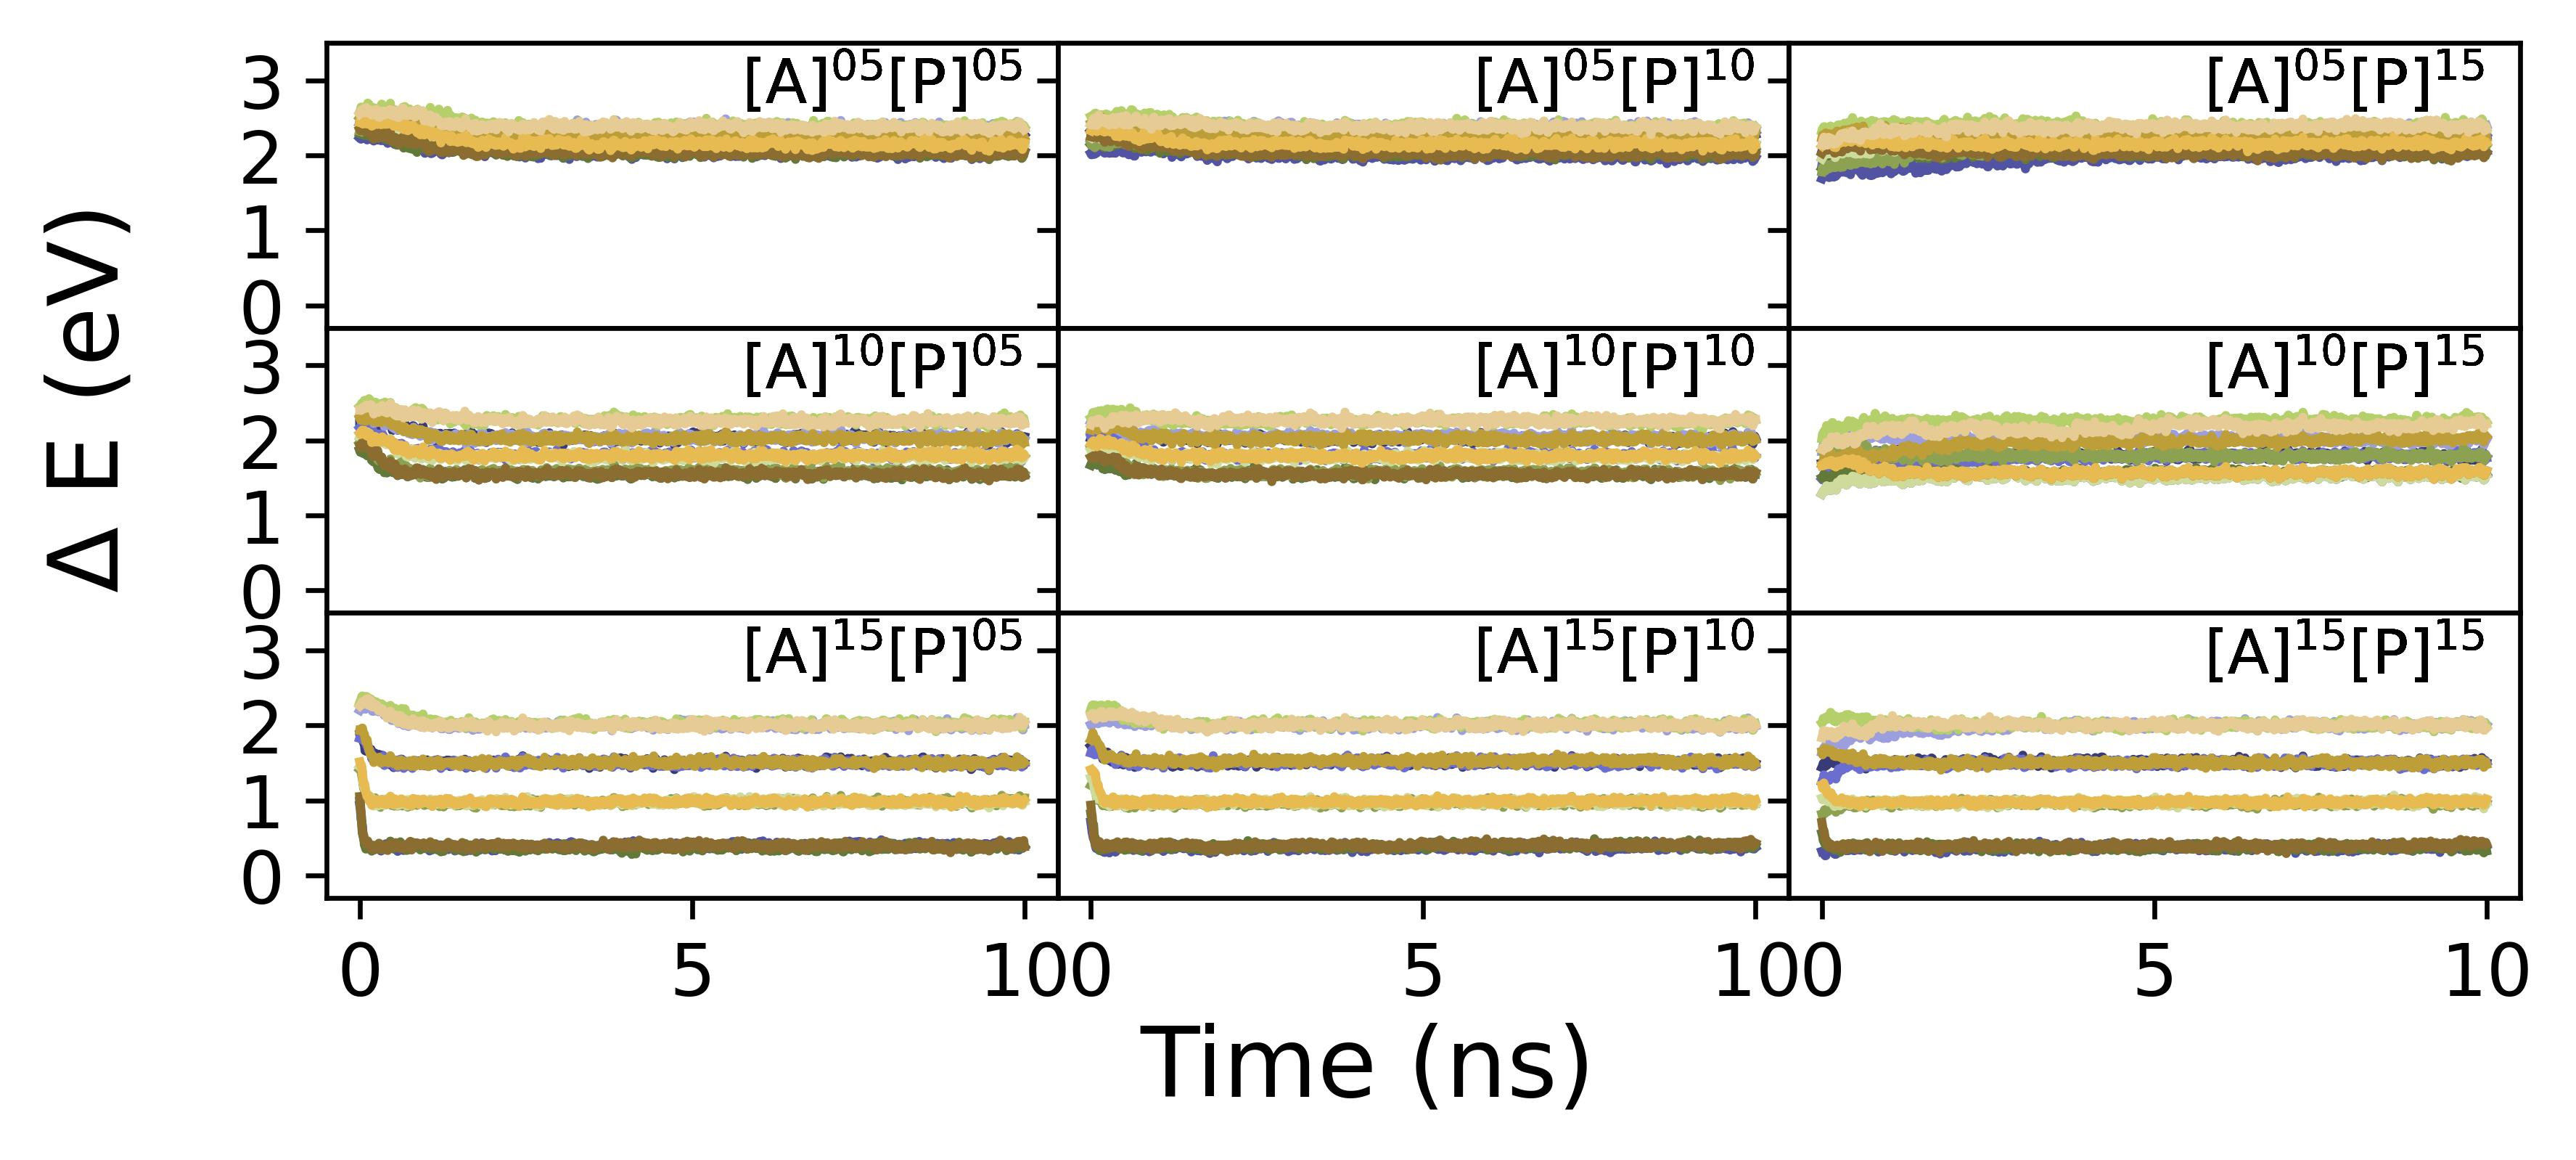
\includegraphics[width=\textwidth]{figures/MD/Env/Jan75_EDelta.jpeg}
\end{subfigure}
    \caption{$\Delta E$ plotted versus time for the various environment parameters tested on the Janus chemical ordering. Each sub-figure presents all time series for a given specified morphology and shares common line colour schemes and axes. Each block is for the given $\rho_{Au}\rho_{Pt}$ parameters, and each line represents a pair of $\varepsilon_{Au}\varepsilon_{Pt}$ coupling strengths. The top three panels are for the 75\% Pt loading. The next three panels are the 50\% Pt loading. The final three are 25\% Pt loading.}
    \label{fig:Delta_E_Env_jan}
\end{figure}

We see a similar patter of behaviour for the Janus configuration wherein if the environment interacts more strongly with Au than with Pt, there is always a decrease in $\Delta E$ which is indicative of the total energy tending towards the cohesivity of the nanoalloy suggesting that there may indeed be relaxation triggered by Au covering the Pt. Conversely, when the environment interacts more strongly with Pt, there is little observable change in the evolution of this parameter, suggesting that there may be some large scale stability possible. However, we require alternative tools to determine the structural nature of the nanoalloy in these instances. 

\begin{figure}
\centering
\begin{subfigure}[b]{0.8\textwidth}
    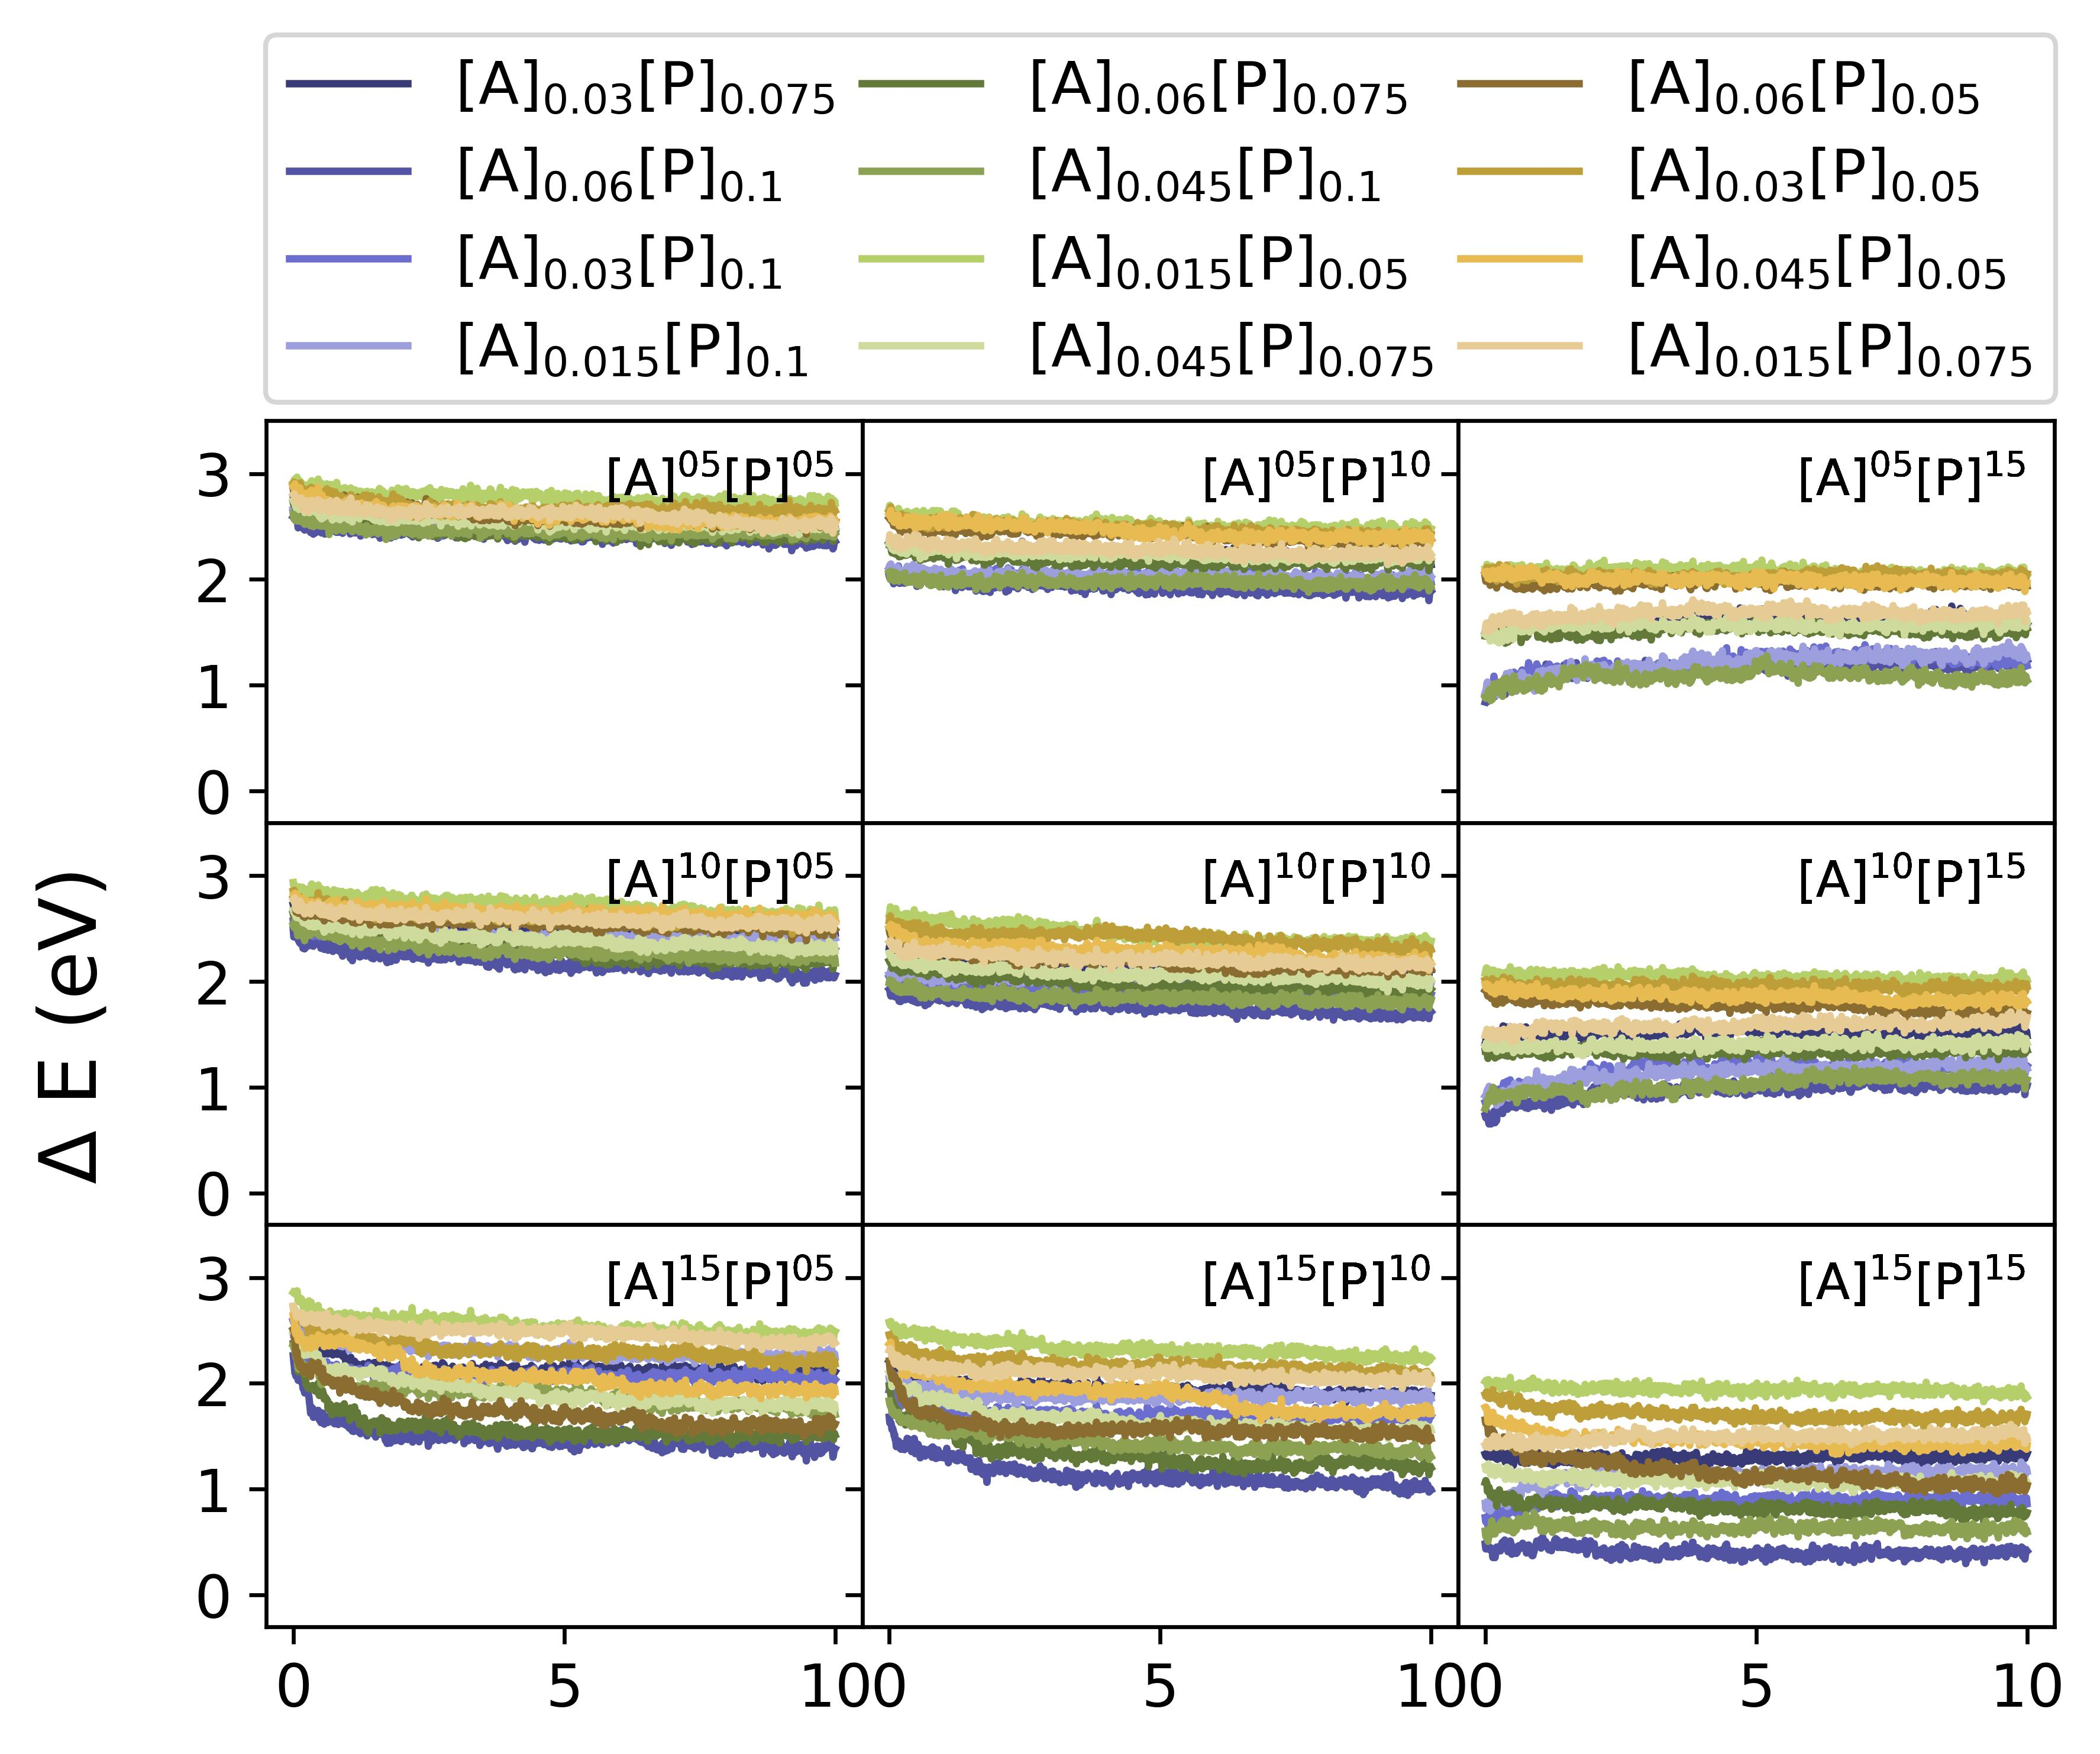
\includegraphics[width=\textwidth]{figures/MD/Env/Rnd75_EDelta.jpeg}
\end{subfigure}\\
\begin{subfigure}[b]{0.8\textwidth}
    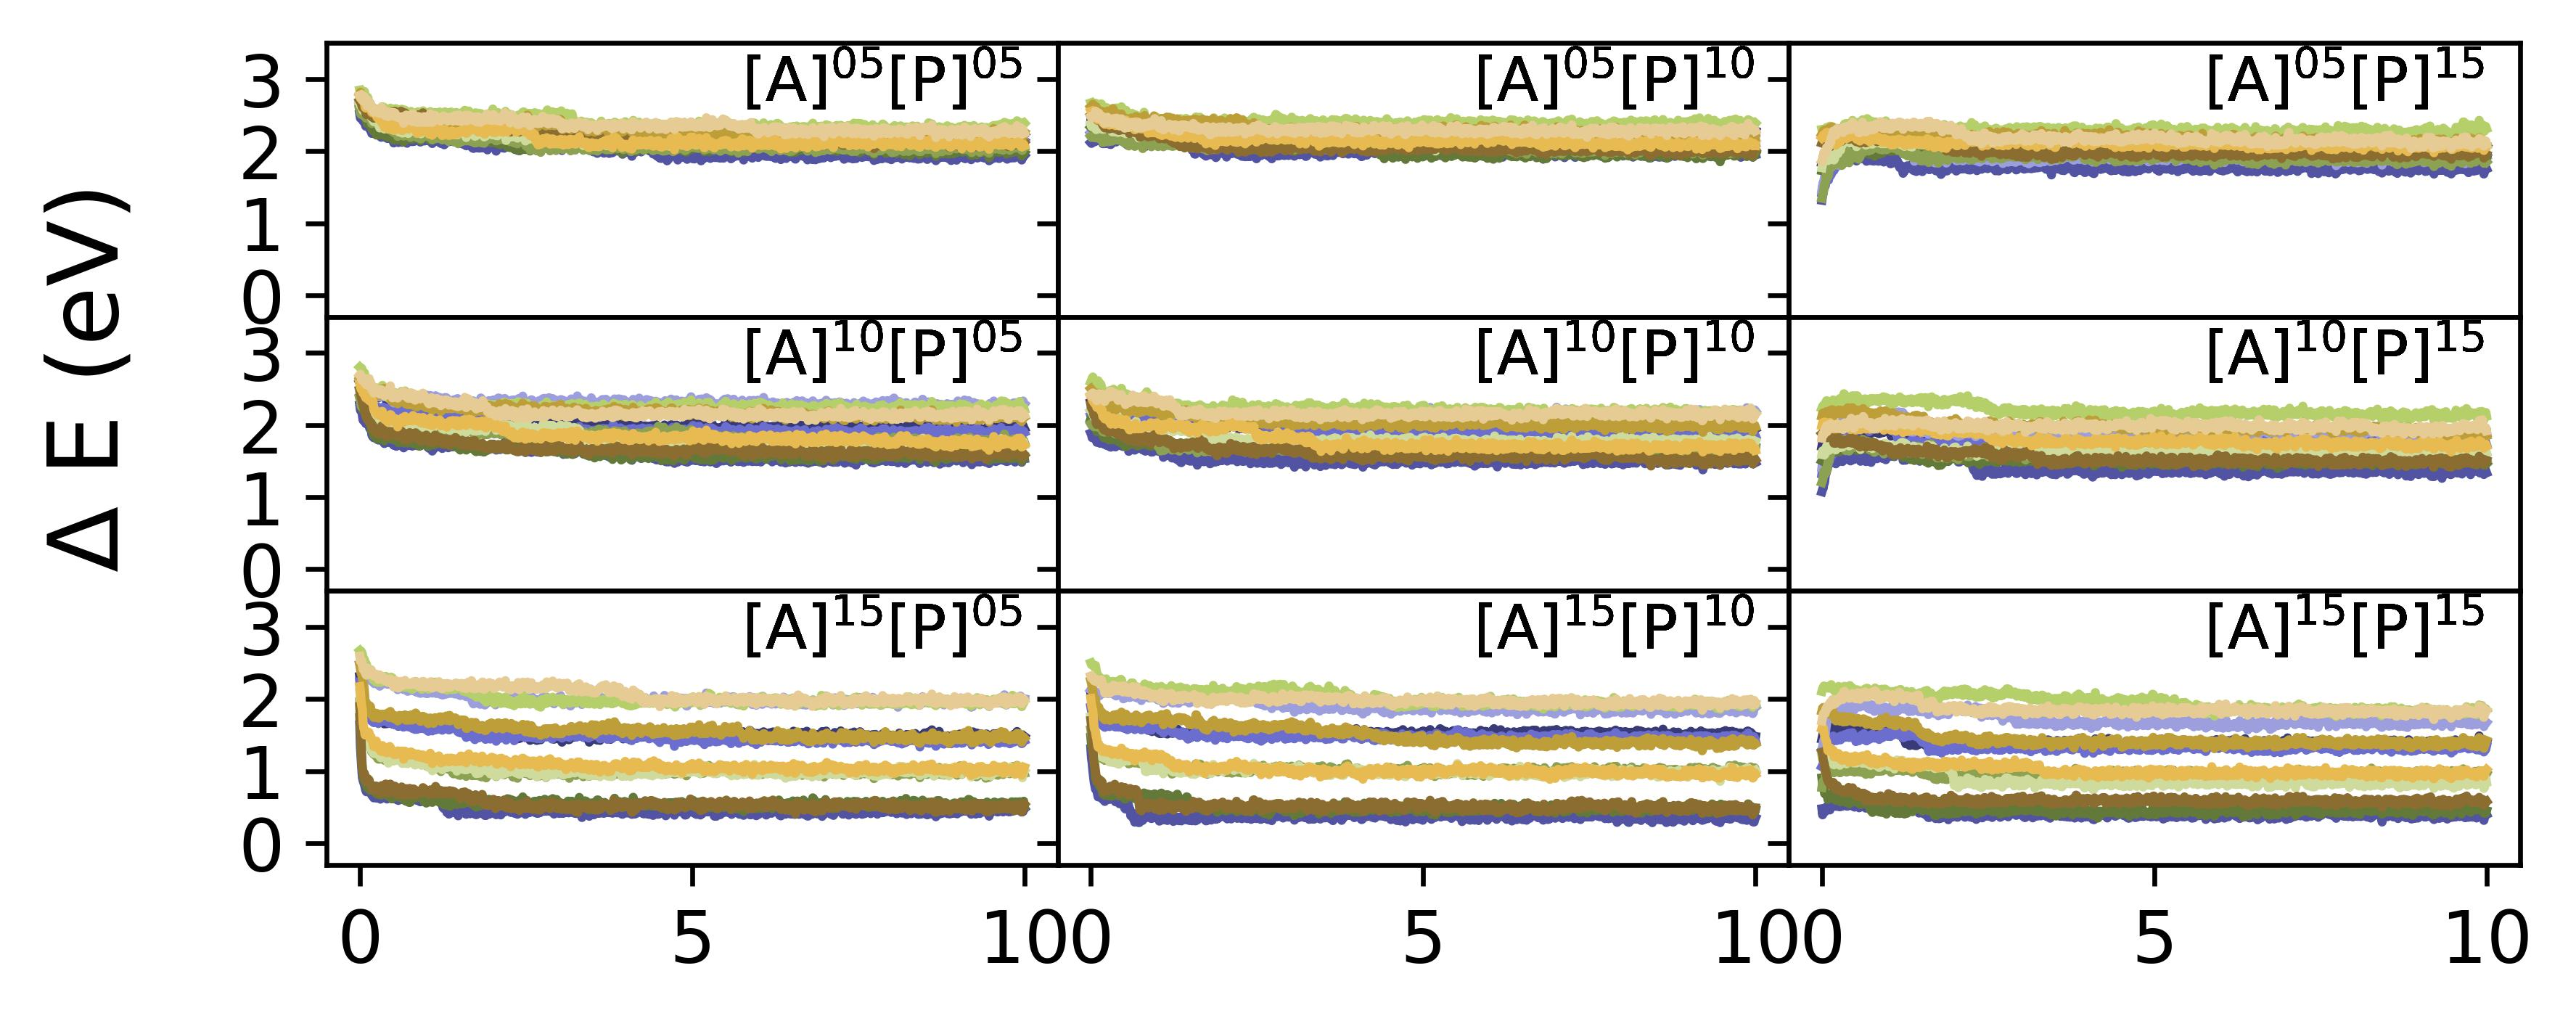
\includegraphics[width=\textwidth]{figures/MD/Env/Rnd50_EDelta.jpeg}
    \end{subfigure}\\
\begin{subfigure}[b]{0.8\textwidth}
    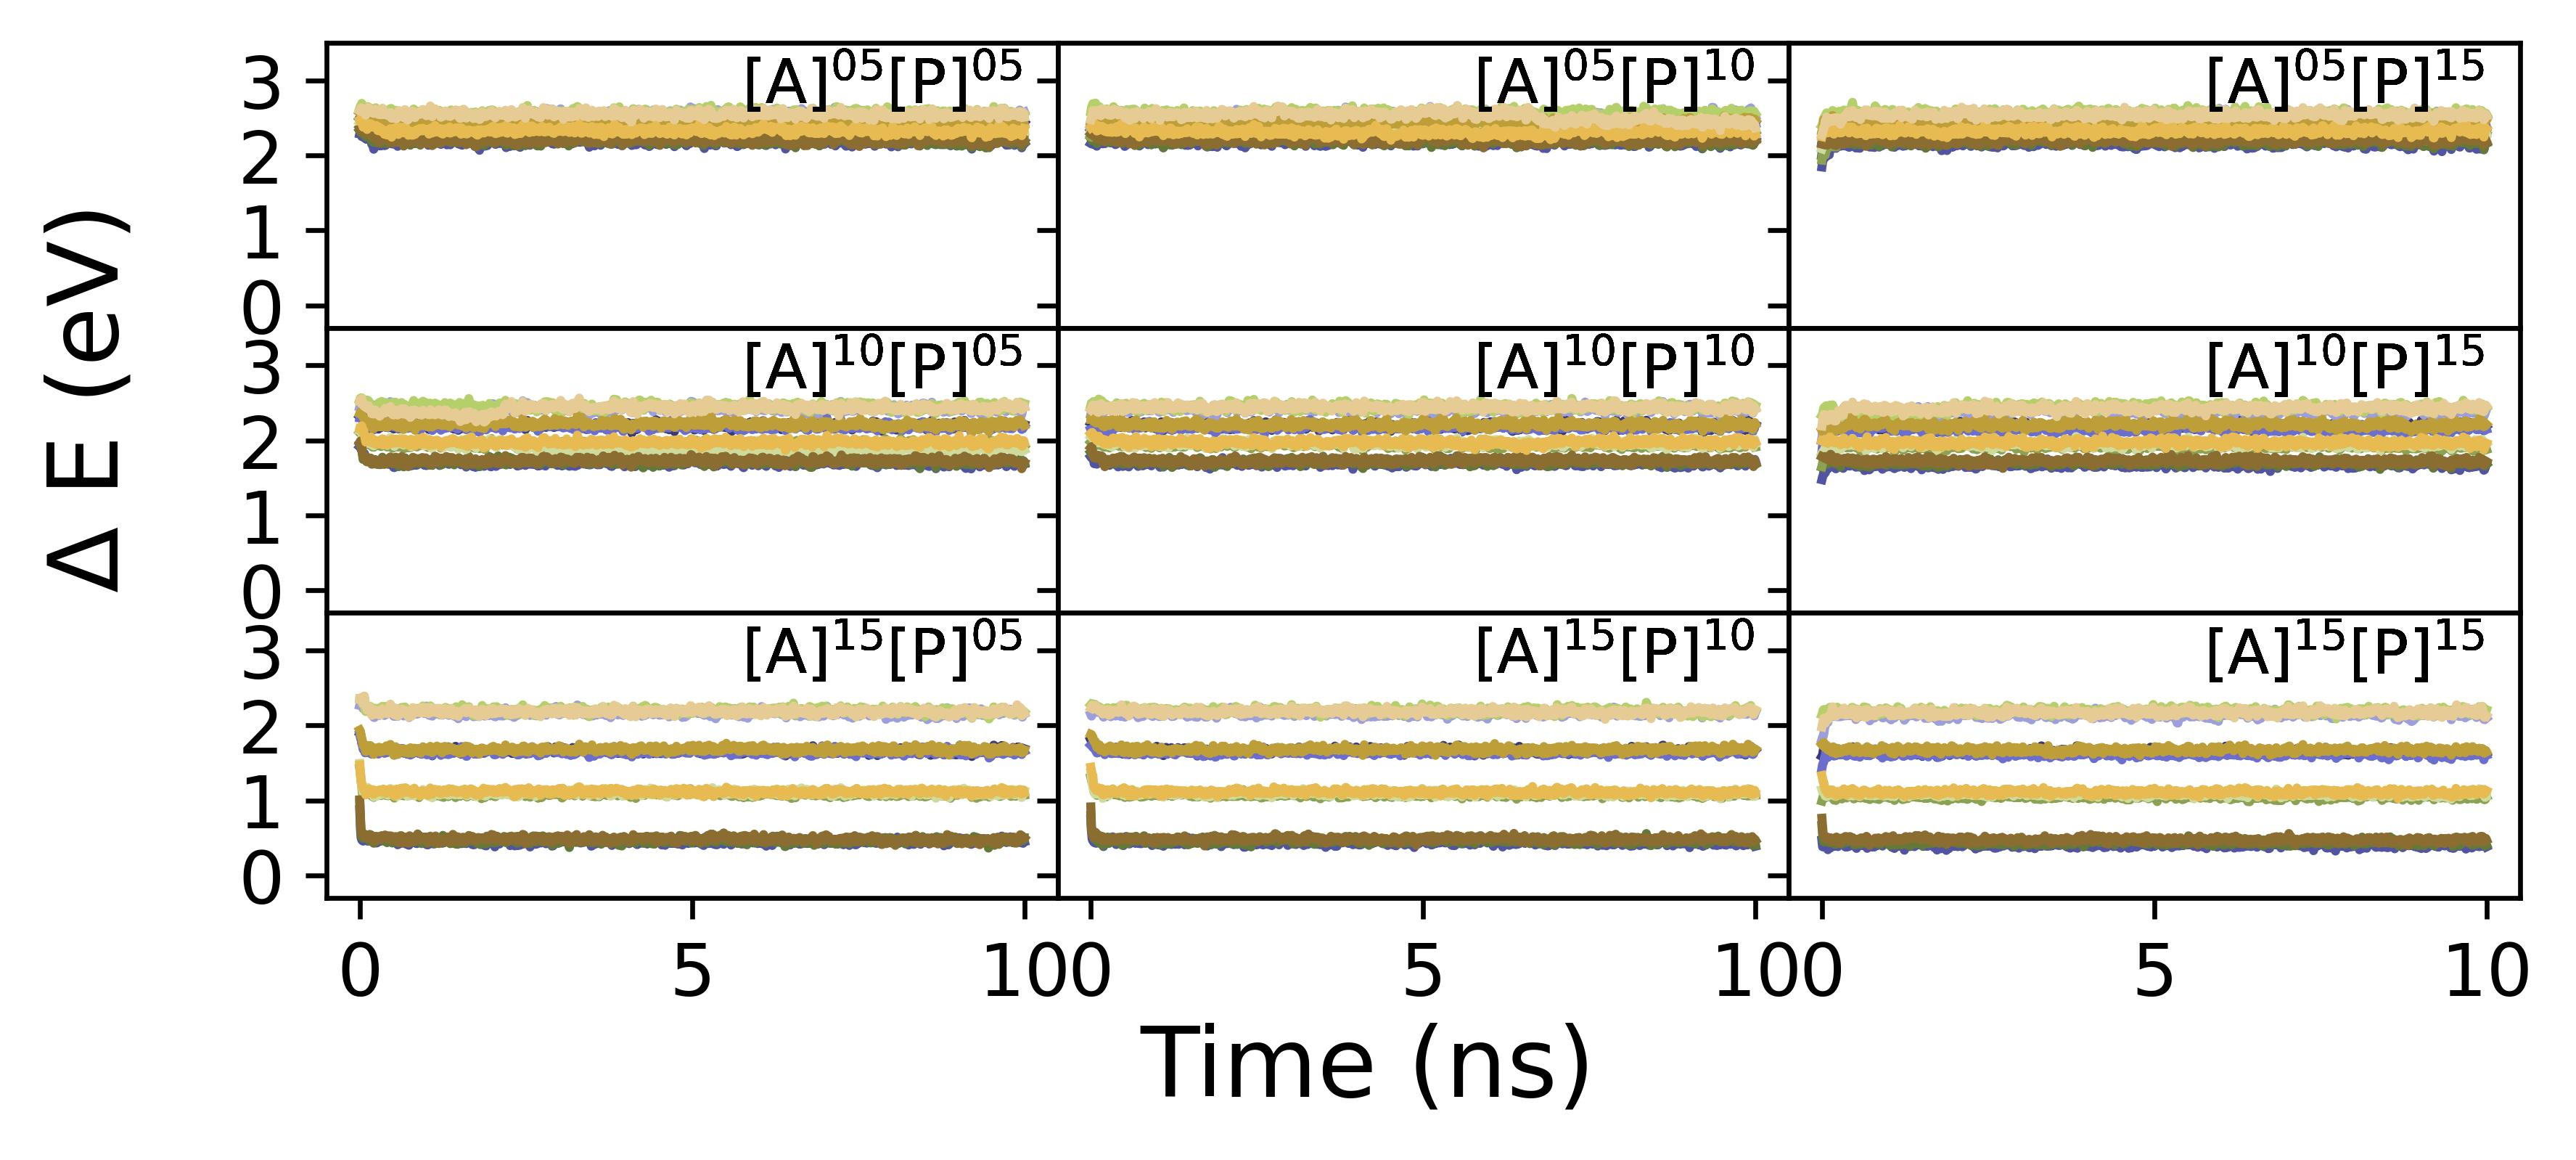
\includegraphics[width=\textwidth]{figures/MD/Env/Rnd25_EDelta.jpeg}
\end{subfigure}
    \caption{$\Delta E$ plotted versus time for the various environment parameters tested on the randomly mixed chemical ordering. Each sub-figure presents all time series for a given specified morphology and shares common line colour schemes and axes. Each block is for the given $\rho_{Au}\rho_{Pt}$ parameters, and each line represents a pair of $\varepsilon_{Au}\varepsilon_{Pt}$ coupling strengths. The top three panels are for the 75\% Pt loading. The next three panels are the 50\% Pt loading. The final three are 25\% Pt loading.}
    \label{fig:Delta_E_Env_rnd25}
\end{figure}

Next we consider the randomly alloyed regime, which from an energetic perspective appears to be effectively the same as was observed for the Janus. Suggesting that the only chemical ordering which is unique in its energetic evolution is indeed the Core-Shell type configuration. As explored in Chapter \ref{c:Alloy}, this should not be surprising as we found that in general it is the large relative abundances of Pt required to form the shell that enable it to be especially stable and capable of resisting large scale migration of Au to the surface.

\subsection{Pt surface contributions}

\begin{figure}
     \centering
      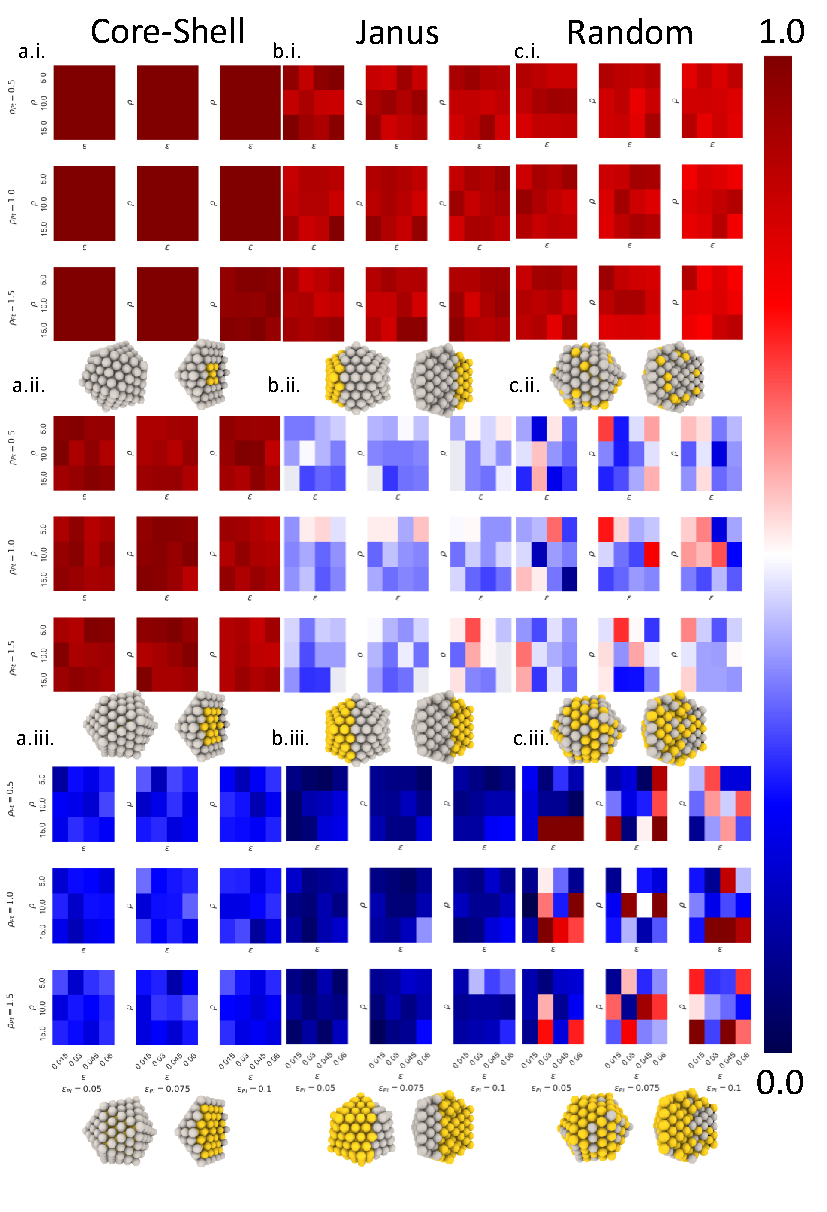
\includegraphics[width=0.9\textwidth]{figures/MD/Env/PtSurf_Env.pdf}
    \caption{Pt surface maintenance heat maps for all of the variations of environment parameters tested. Each grid block corresponds to a fixed Pt environment with the exponent varying down the rows and the interaction strength varying across the columns. Each grid of $9$ blocks corresponds to every permutation of interaction parameters for a given morphology - as depicted below each grid with the corresponding structure and its cross section. Each individual cell is assigned a colour based on the ratio of Pt$_{Surf}(t_{f})/$Pt$_{Surf}(t_{f})$.}
    \label{fig:PtSurf_Env}
\end{figure}

In figure \ref{fig:PtSurf_Env} we present the survival of Pt at the surface as the primary characteriser for the environment parameters considered. To compute the colour of each cell, we consider the ratio between the number of surface-like Pt atoms at the end of the brief dynamics to those at the beginning. We have purposely scaled this to exist in the unit interval as we are solely concerned with the loss of available Pt surface for catalytic reactions to occur upon.  Whilst it is possible in the instances of a high Pt ratio and an environment strongly coupling to Pt that there may be more Pt atoms brought from the interior to diffuse across Au, this is more a corollary of the observation that Pt may indeed be stabilised atop Au under some conditions. That is to say that it is a possible extreme example of the general behaviour we intend to observe. However, it is unlikely that this is indeed occurring when one considers the top blocks of Figure \ref{fig:PtSurf_Env}. In the example of the Core-Shell morphology, the surface is initialised with a saturation of Pt with the only route to introducing further Pt surface-like atoms being the trivial instance of the surface becoming disordered at finite temperature. Alternatively, one may interrogate the example of 75\% Pt composition in the Janus structure. In this example, we explicitly see that there are no examples of a dark red hue in the heat map suggesting that we are indeed losing viable Pt surface. Likewise, the same may also be said for the randomly mixed alloy. That is to say, the justification for considering only on the unit interval for Pt survival is sound.

Indeed, a reflection on Figure \ref{fig:PtSurf_Env} reveals some striking and interesting quirks within the results. As discussed above, the examples of overabundance of Pt trivially results a in larger recoverable Pt surface. This too is evidenced even in the vacuum case as seen in Figure \ref{fig:Ptload_Data} whereby we observed that a larger incoming Pt decoration resulted in a larger viable Pt surface remaining. However, we do note that for some parameter sets, it is possible to maintain a finite quantity of surface-like Pt atoms. Of particular note is in the example of randomly alloyed structure wherein we observe that for all values of the coupling energy $\varepsilon_{Pt}$ there are instances in which an appreciable amount of Pt remains at the surface. Where the interaction type is weak and covalent-like with $\rho_{Pt}=0.5$, paradoxically a stronger Au interaction type is required to keep the initial Pt where it is. It is possible that given the combination of large coupling energy $\varepsilon_{Au}$, interaction type $\rho_{Au}$, and the lack of Pt in general that the Au is essentially fixed in place by the environment, arresting the necessary atomic motion for Pt to move interstitially and become encapsulated by the Pt. A phenomenon we indeed see evidence for weaker Au-Environment parameters in the very same block.

Furthermore, upon comparison of the random mixing with Janus chemical ordering, we observe that whilst there are in principal an equivalent number of initial surface like Pt atoms between the two configurations it would appear that the latter behaves poorly independent of the environment type with respect to maintaining a Pt population at the surface. One could make the argument that the relative homogeneity in the Janus phase is what permits the active mobility of Au to coat the Pt, in that there may be a concerted directionality in moving material from surface and sub-surface sites of the Au component of the Janus towards the Pt side. 

We may also return to the comment regarding the similarity in the energetic profiles of both the Janus and randomly alloyed clusters and map it to the same observation from the perspective of Pt surface contributions. In general, the two columns of Figure \ref{fig:PtSurf_Env} representing these chemical ordering configurations are reminiscent of one another in a similar fashion as the two profiles of $\Delta E$ for the same clusters. That suggests that they may dynamically behave in a similar fashion too, which was explored for a broader class of nanoallloys in Chapter \ref{c:Alloy} where we came to similar conclusions. That when one alloys metals of two strongly varying cohesive energies, one may expect a degradation of the surface presented by the more cohesive metal in favour of forming a greater surface of the less cohesive specie. Whilst there is a clear indication that having a strongly interacting environment with the more cohesive metal permits the preservation of some of the initial surface, this only really appears to be a perturubative effect and not as strong as perhaps anticipated. We argue this given the slightly lighter tiles in the bottom right hand corner for each block of Figure \ref{fig:PtSurf_Env} which means that there exists a sufficiently non-zero contribution of the Pt to the surface.

Now we wish to address the bottom right 3$\times$3 block of Figure \ref{fig:PtSurf_Env} representing the 25\% Pt loaded randomly mixed nanoalloy. It would initially appear that this may be particularly effective at maintaining an appreciable Pt population behaving surface-like. However, this is likely an effect of the entire cluster behaving as a liquid drop with the lack of a large cohesive Pt region acting as an anchor for mobile Au atoms to move across. Indeed, as we saw in Chapter \ref{c:Alloy}, the temperatures modelled here are sufficient for the cluster to undergo a partial melting, especially at the small sizes modelled. Given that we have not performed any annealing process, then it may be that in this liquid drop phase, Pt is able to be unintentionally left sufficiently uncoordinated to be considered surface-like due to the churning of the atoms. Indeed, it would be a natural extension to this investigation to consider the annealing of each cluster subject to the same environmental parameters as they were during the NVT dynamics.

\subsection{Discussion}

Introducing a solvent model to a dynamical system is never a simple task, as there are a number of factors to be considered and weighed up. Moreover, it cannot be guaranteed that a given solvation model for one set of inter-atomic potentials will yield physically meaningful results when paired with another set for which they have not been rigorously tested. Therefore, the model we have selected is indeed one which was designed with the SMATB potentials directly in consideration, which conveniently aligns with our objectives in introducing a solvent implicitly to our classical dynamics presented in Chapter \ref{c:Coal} and Chapter \ref{c:Alloy}.

To begin a preliminary investigation into the efficacy and functionality of this new model, we first considered the effects that altering the parameters would have on the pure Au and pure Pt cases as a form of bench-marking. Having rationalised these results and verified that they were sufficiently sensible given the range of parameters considered, we proceeded to introduce a series of small AuPt clusters of varying chemical ordering and Pt loading - verifying against the AuPt data from Chapter \ref{c:Alloy} and searching for evidence of their efficacy.

Indeed it appears that by having a strongly interacting environment-Pt parameterisation with a covalent or pair-wise interaction with Au, we are able to appreciably influence the surface composition. This is encouraging for two reasons. First, it is intuitively reasonable for this to be true, and adds further weight to the utility of this solvation model at the classical level - even more so when we factor in its relatively low computational overhead. Second, it provides us with a starting point from which we may begin to search for solvents which behave in this precise way, and indeed probe the interaction of commonly used solvents, for example water, with these nanoalloys so that we may approximately map the interaction type and strength of these solvents with Au and Pt separately and in composite. This is precisely the spirit of the multi-scale modelling approach which we wish to utilise for the purpose of this project.

By continuing to explore the utility and efficacy of the implicit solvation model through the application to larger, more complex systems and on longer time scales, we may further develop our understanding of the interactions of nanoscale systems interacting dynamically with an arbitrary environment. This will help in facilitating a more comprehensive understanding of nanoscience in strongly interacting environments.

\section{The effect of water on AuPt nanoalloys}
\label{sec:H2NA}

\subsection{Water - Pt adsorption energies}

As a corollary to the simulations previously discussed \ref{sec:AuPt_DFT}, we have proceeded to perform a set of dynamics and energetic evaluations following the adsorption of a single water molecule. Such water molecule is adsorbed atop the Pt dopant on Th$_{20}$ isomer. We perform the Quickstep routine of \texttt{CP2K}, atomic basis sets of the form "DZVP-MOLOPT-SR-GTH", and an energy cutoff of 400 eV to get a quick and efficient evaluation of energies, as well as of their electrostatic properties. To account for the additional Van der Waals (long range) interactions, we used a dispersion interaction of the form Grimme DFTD3 \cite{Grimme_D3_2017}  which are likely to exist between the water and the nanoalloy but have otherwise been neglected between metallic species and Jellium in Chapter \ref{c:L-M}.  A cubic unit cell was set to be 20 \AA \ in each dimension with the cluster-molecule system at the centre. We maintained this cell size for all of the considered structures so as to be consistent when reporting the energy of the system in each instance.

\begin{figure}[ht!]
    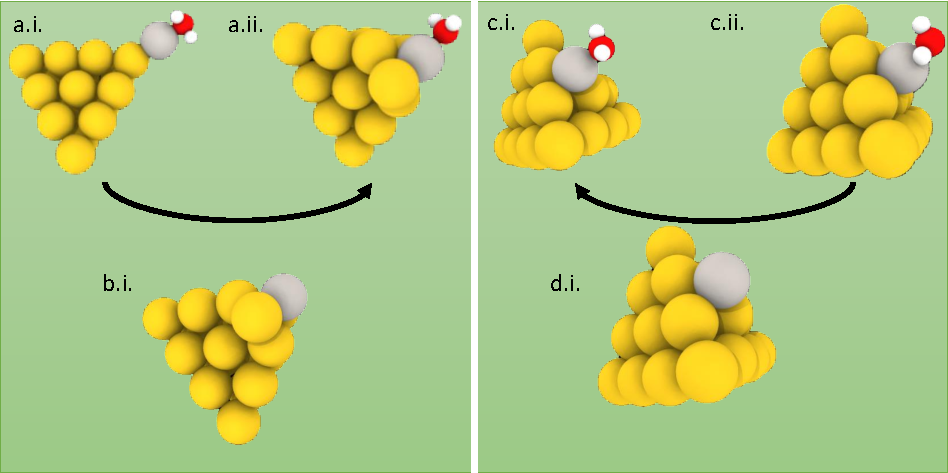
\includegraphics[width=15cm]{figures/LM/AuPt_EPJ/AuPt_Wet.pdf}
    \caption{Graphical illustrations of the systems evolved. \textbf{a.i.} is the initial configuration of H$_2$O adsorbed atop a Pt atom itself adsorbed atop Au$_{20}^{Th}$. \textbf{c.i.} Is likewise for H2O adsorbed atop a Pt atom deposited onto the side of Au$_{20}^{Th}$. Subsequently, sub-panels \textbf{a.ii.} and \textbf{c.ii.} are the resultant structures following a 2 ps dynamical AIMD simulation at 600 K. Panels \textbf{b.} and \text{d.} are the structures with water stripped away.}
    \label{Fig:cp2k_water}
\end{figure}

We present in Figure \ref{Fig:cp2k_water} the configurations considered for an initial investigation into the explicit introduction of water molecules to small systems of AuPt. Given that we only consider a single molecule when the cluster is 21 atoms in size, with essentially the entire structure being surface like, one may consider this environment to be humid rather than solvated. However, the introduction of a single molecule permits us to more easily recover the adsorption energy for each adatom example presented. We discuss later in this chapter the considerations which may be made when greater amounts of water are considered.

We note already that the introduction of water has caused the displacement of the tip Pt decoration where this was previously considered to be stable. Indeed, a facsimile verification simulation was run to confirm that a Pt atom adsorbed atop the Au$_{20}^{Th}$ is structurally stable. As previously we had only verified this with the SMATB potentials and the geometry optimiser built into \texttt{Octopus}. Essentially, we wished to verify that this new geometry was not unique to \texttt{CP2K} and its set of potentials and protocols for computing forces and implementing geometry optimisation. Indeed, this destabilisation of the structure appears to be solely due to the presence of water. Conversely, such a restructuring was not observed when Pt was adsorbed on the central face of the Au cluster. In principle this should not be surprising at it has already been established within the context of simulations subject to the SMATB potentials that Pt has a propensity to maximise its number of Au neighbours where possible. Finally, one must also recognise that such a configuration with Pt behaving like an antenna can only be meta-stable when being optimistic - and it stands to reason that the perturbing influence of an adsorbed molecule is sufficient to push the structure into a more stable structural conformation.

\begin{table}[ht!]
\centering
\caption{Energy profiles of water adsorbed on AuPt NPs. Computed with \texttt{CP2K} \cite{cp2k_2020}.}
\label{tab:ads_cp2k}
\begin{tabular}{@{}lll@{}}
\toprule
Structure & |E$_{GS}$| (eV) & |E$_{ads}$ (eV)|     \\
\hline
Au$_{20}^{Th}$Pt$_{1}^{Tip}$           & $21.27556\times10^{3}$ & N/A    \\
Au$_{20}^{Th}$Pt$_{1}^{Face}$          & $21.27539\times10^{3}$ & N/A     \\
H$_{2}$O                               & $466.9001$ & N/A    \\
Au$_{20}^{Th}$Pt$_{1}^{Tip}$H$_{2}$O   & $21.74314\times10^{3}$ & $0.673$     \\
Au$_{20}^{Th}$Pt$_{1}^{Face}$H$_{2}$O  & $21.74298\times10^{3}$ & $0.682$    \\
\bottomrule
\end{tabular}
\end{table}

We present in Table \ref{tab:ads_cp2k} the computed total ground state energies for each of the systems and the corresponding adsorption energy of water where appropriate. We have simply determined these adsorption energies to be the defect remaining when one considers the sum of the energies of the isolated systems against the energy of the composite system.

\begin{equation}
    E_{ads} = E_{Solvated} - \left( E_{H_{2}O} + E_{NA} \right)
    \label{eqn:adsorbed}
\end{equation}

This is formally formulated in Equation \ref{eqn:adsorbed}, where the adsorption energy is computed precisely as described above. 

Initially, we must perform a reality check on our results prior to further discussion. A precursory comparison with existing literature reveals a broad range of accepted values for different types of extended Pt surface \cite{C8RA00952J,doi:10.1021/jp201608x,C8SC02495B} and Pt nanoparticles \cite{doi:10.1021/acs.jpcc.9b06136}. In general, we may consider a reasonable value for the adsorption energy of water on Pt to be in the range of 0.4 eV to 0.8 eV where there are reasonable examples of values both higher and lower than this range depending on the geometry considered. Nonetheless, given that our values are approximately in the centre of this range, we may consider them to be faithful in the capacity that our DFT investigation permits. Moreover, there does not appear to be a particularly rich section of preexisting investigations into AuPt nanoalloys interacting explicitly with water indicating the novelty of this study.

\begin{figure}
\centering
\begin{subfigure}[b]{0.425\textwidth}
    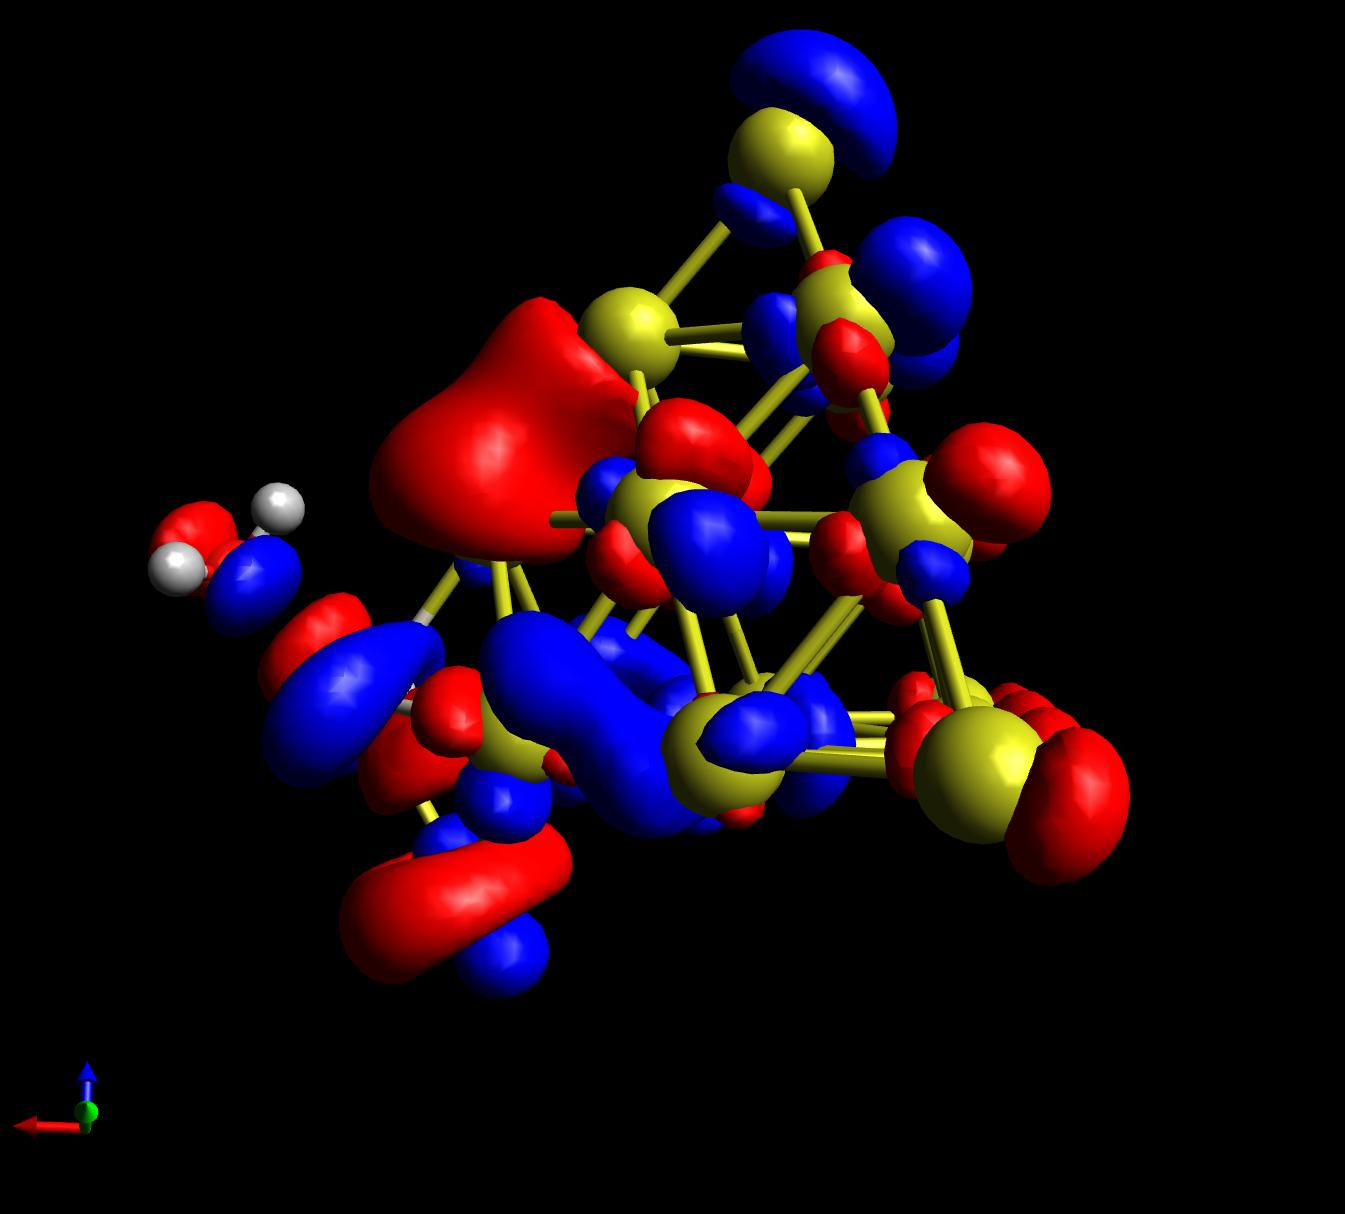
\includegraphics[width=\textwidth]{figures/ThTip_NVE-WFN_00123_1-1_200.jpg}
    \caption{Tip configuration HOMO orbital.}
    \label{fig:tip_wfn}
\end{subfigure}
\begin{subfigure}[b]{0.425\textwidth}
    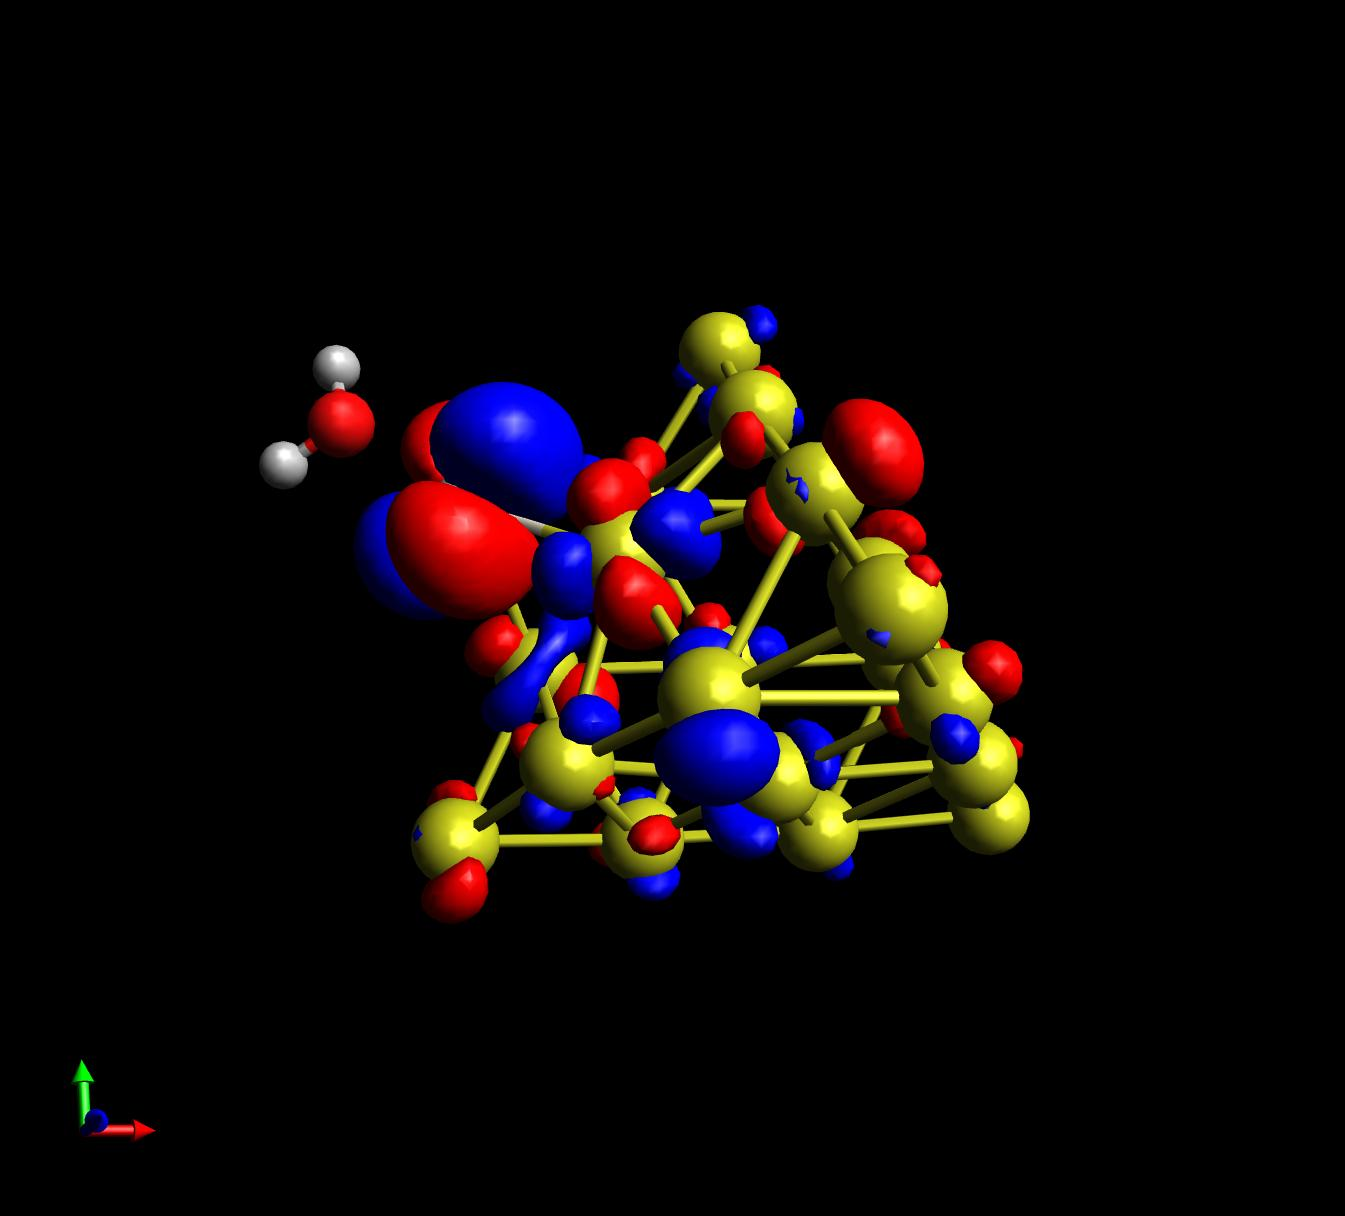
\includegraphics[width=\textwidth]{figures/ThFace_GO-WFN_00123_1-1_202.jpg}
    \caption{Face configuration HOMO orbital.}
    \label{fig:face_wfn}
\end{subfigure}
    \caption{Iso-surface 0.02 representations of the HOMO for both configurations considered. Computed using QUICKSTEP \cite{QuickStep} in CP2K \cite{cp2k_2020}. Both structures relate to the geometrically optimised configurations referenced in Table \ref{tab:ads_cp2k}.}
    \label{fig:Water_Wfns}
\end{figure}

One may observe that the face-adsorbed configuration has a marginally greater water adsorption energy when compared to that of the tip site. One may make the argument that the face-type configuration has a larger semi-local Au environment to stabilise the water molecule as it is not unlikely that there will be a finite amount of bonding between the adsorbed molecule and the support-like Au nanoparticle. Conversely, even following geometrical optimisation, the tip configuration has a small base for Au support to interact with the water, which may be the causal factor for a slightly smaller adsorption energy.

Furthermore, we may consider the HOMO orbitals for each of the systems presented in Figure \ref{fig:Water_Wfns} and remark that these orbitals are indeed centred on and around the Pt inclusions - consistent with the observations made in Chapter \ref{c:L-M} with respect to the inert structures' PDoS where we demonstrated that the $d$ type orbitals of Pt were centred at and around the HOMO-LUMO region of the nanoalloy. Indeed this is precisely what we see  in the aforementioned figure where there is a strong $d$-type contribution to the wavefunction localised around the Pt in both instances. Moreover, where we have deposited the Pt inclusion on the tip of the Au$_{20}^{Th}$, we see that there is an appreciable overlap between the wavefunction localised around Pt and the water - indicating that that the HOMO state is a covalent bond between the Pt and the adsorbed water as seen in Figure \ref{fig:tip_wfn}. Conversely, we see that when the Pt is adsorbed onto the face of the Au$_{20}^{Th}$ in the presence of a nearby water molecule, the HOMO state in Figure \ref{fig:face_wfn} is almost exclusively localised as a $d$-type orbital centred on Pt and does not overlap with water. By referring back to Figure \ref{Fig:AuPt_PDoS}, we see that the $d$-orbital structure around the HOMO-LUMO region of both considered AuPt nanoalloys exhibit stark deviations in their structure. In the instance of the adatom being on the tip, we reported that the Pt contribution to the PDoS was greatly smeared out across the available energy as low as 5 eV below the HOMO followed by a small $p$-type contribution at 2 eV into the unoccupied states. Compared against Pt as a tip adatom where there was still evidence of the Pt contributing to lower lying states and unoccupied states, the pre-eminent contribution was directly at and up to 1 eV below the HOMO state. Therefore, it should not be surprising to observe the HOMO states being localised around Pt, albeit with contributions localised around many of the Au atoms of the nanoalloy, what is curious is that there appears to exist this overlap in states between the water and the Pt. We stress here that such a property is encouraging from the perspective of catalysis, as if there exists a high energy state shard between water and Pt, it will be more likely that hot holes may be more easily excited from this state - thereby facilitating catalysis.

Indeed, it is our intention to expand the scope of this investigation to more fully consider the phase space occupied by ultrasmall AuPt nanoalloys interacting with water. We began this study by considering two model examples of structures from Section \ref{sec:AuPt_DFT}, which presented in Reference \cite{JonesAuPt} the variation in structural, static, and optical properties of these ultrasmall alloys, indeed we would like to complete the search of the space identified here whilst considering alternative adsorption sites in a systematic fashion so as to more comprehensively describe the AuPt - water adsorption map. Already these early results are encouraging from the perspective of catalysis, as we have begun to develop a map of adsorption energies from water interacting with AuPt nanoalloys and are able to explore the properties of the HOMO orbitals which, given their location in the local energy landscape, have a higher probability of contributing to electron~-~hole excitations.

\subsection{Solvated AuPt nanoalloy}

We now consider the dynamics of a more earnestly solvated nanoalloy. We have elected to consider the Au$_{13}^{Ih}$Pt$_{42}^{Shell}$ for its ubiquity in this thesis insofar and the reasons previously given to motivate its use. Indeed, we have already performed a small DFT investigation in Sec. \ref{sec:Res_Atom} within the simplified LDA to describe its static and optical properties - comparing them with the isolated components. Here, we extend this description by considering its ultrafast dynamics within the \texttt{CP2K} package when expose to 20 water molecules. Solvation was achieved by identifying a thin spherical shell between the spherically approximated surface of the nanoalloy and a further nanometer beyond this to permit the variation in orientation and relative distance to the structure for each introduced water molecule. We then proceeded to randomly populate this shell with 20 water molecules, ensuring no overlap as they were placed. This number of molecules was arbitrary in its exactness; however its size is appropriate given the dynamics we wish to monitor and the consideration for computational resources which are known to scale poorly with system size at the \textit{ab initio} level of theory.

An optimisation of the geometry was performed prior to beginning dynamics to assist with the convergence of the forces computed during the 13 fs of NVT dynamics at 600 K. Whilst it would be desirable to have a longer trajectory from which we may make statistical inferences, computational constraints have presented us with the unique opportunity to more finely consider the initial moments of dynamical motion of an explicitly solvated AuPt nanoalloy. As discussed above, a phenomenon infrequently observed.

\begin{figure}[h!]
    \centering
    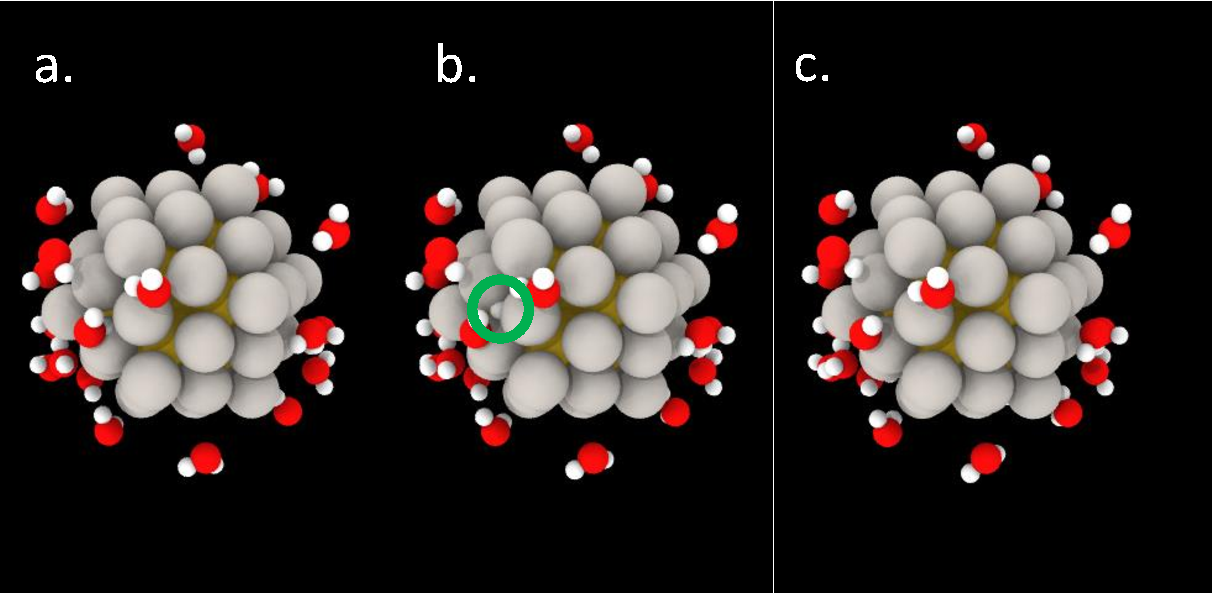
\includegraphics[width=0.9\textwidth]{figures/AuPtSolv.pdf}
    \caption{Aqueous AuPt Core-Shell nanoparticle interacting with explicit water. (\textbf{a}) Is the intitial solvation. (\textbf{b}) is after 8 fs where the green ring is highlighting a mobile H atom. (\textbf{c}) Is the final system following the brief dynamics.}
    \label{fig:CS_Solv_im}
\end{figure}

We show in Figure \ref{fig:CS_Solv_im} the aqueous AuPt system selected for the brief study. We have included 20 water molecules to form the solvent, a sufficient amount to collect statistics, but not too many as to be prohibitively computationally expensive for a preliminary investigation. Whilst there is not great evidence of structural changes in the nanoalloy on such fast time scales, we are able to observe in (\textbf{b}) of the figure that a single H specie has become detached from its parent oxygen. Under the proviso that this is indeed the observed mechanism, then the deprotonation of water is deeply encouraging as a result. Nonetheless, for such a brief set of dynamics, and given the random fashion in which we have solvated our nanoalloy, it is necessary to perform further studies with longer dynamics to gather more statistics regarding this event. Nonetheless, it is sufficient evidence of the affinity which H has with Pt which has identified Pt as such a promising catalyst for the water splitting reaction.



\begin{figure}
    \centering
    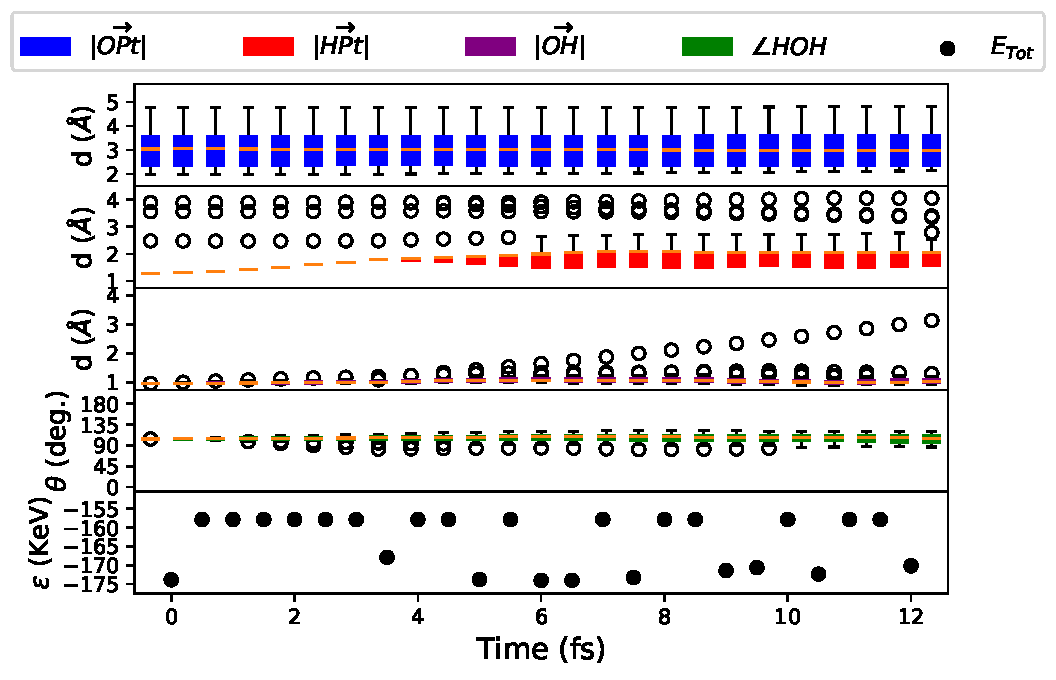
\includegraphics[width=0.95\linewidth]{figures/CS_Solv.pdf}
    \caption{Initial snapshot of dynamical properties of a CS AuPt NA solvated within $20$ water molecules. Top panel presents box plots of the O-Pt bond distance with the red line in each box identifying the mean position, circles are points greater that $1.5$ times the standard deviation of all distances above the mean. Middle panel are box plots showing the distribution of characteristic water angle $\angle HOH$ with the orange line in each plot depicting the mean angle. Bottom panel is the total energy of the system at the given time frame.}
    \label{fig:CS_Solv}
\end{figure}

Even with only a short time frame of 13 femtoseconds available for analysis given computational constraints, it already possible to make observations and draw conclusions from Figure \ref{fig:CS_Solv}. Initially, we note in the $3^{rd}$ row illustrating the evolution of the $\angle HOH$ bond angle that the average angle is tightly localised around 104$^{\degree}$ compared to the natural angle of 104.5$^{\degree}$ which is already encouraging. Whilst this offset appears to be consistent throughout the brief dynamics, the uncertainty depicted by the size of the box plot for each point grows slowly in time. Suggesting that the presence of the nanoalloy is causing the hydrogen to act under the influence of the larger object. Indeed, we may observe in the provided snapshots of Figure \ref{fig:CS_Solv_im} that several hydrogen atoms are drawn towards and even into the nanoalloy. This observation is further corroborated by the data in the $2^{nd}$ and $3^{rd}$ rows of Figure \ref{fig:CS_Solv} in that we observe initial net repulsion of H with respect to the outer shell of Pt which then begins to reverse after 3 femtoseconds. Recalling that these distances are on the order of 1 to 2 \AA, this distance is approximately consistent with the typically observed H-Pt distance of 1.56 \AA \ \cite{B600250C,https://doi.org/10.1002/anie.201813958,doi:10.1021/ja902876v}.

Whilst we have not been able to identify strong signals for the deprotonation event discussed with respect to Figure \ref{fig:CS_Solv_im} in Figure \ref{fig:CS_Solv}, there is sufficient evidence that the presence of the AuPt nanoalloy is not globally influencing too strongly the HOH morphology, there are indicators, principally in the $\vert\overrightarrow{OH}\vert$ presented, that there is a strong tendency for H to move away from its parent O specie whilst moving towards a nearby Pt. That the O is relatively immobile is also seen in the first panel of box-plots in Figure \ref{fig:CS_Solv}. Typically, the $\vert\overrightarrow{OH}\vert$ bond length is 0.97 \AA. However, we can see clearly in the 3$^{rd}$ panel of Figure \ref{fig:CS_Solv} the motion of a single H specie being carried away from its original O partner by nearly 4 \AA \ which essentially is motion from the surface to the sub-surface of the cluster.

Whilst these early results are curious with respect to the observed water deprotonation, it is clear that a longer trajectory must be sampled so as to make stronger conclusions regarding the nature of AuPt nanoparticles in a liquid environment. Moreover, we must also vary the morphology of the initial solvent~-~nanoalloy system to ensure that the aforementioned mechanism is not a consequence of an unusually unstable configuration. Indeed, it is highly likely that the observed event is a consequence of the initial conditions of the geometry. Rather, by iterating over randomly solvated systems, we may begin to identify further mechanisms which may be then studied in more precise detail as single site interactions to determine the nature of the potential energy surface at the heart of water splitting on AuPt nanoalloys.

\subsection{Discussion}

In this investigation, we have explored from an \textit{ab initio} perspective the influence that water may have on ultrasmall nanoalloys. This was done to support the investigations into introducing an implict solvation model to the classical molecular dynamics calculations. By learning through \textit{ab initio} methods the energetics of AuPt - solvent interactions, we may be able to have a more parametrically accurate description of clusters in an environment. Moreover, this investigations provides us a direct window through which we may begin to observe the fundamental chemistry at the heart of the water splitting reaction we are investigating in this project. Whilst the results presented constitute early and incomplete data, we choose to present them due to the encouraging results and the discussions they facilitate. It is naturally a future objective to continue these studies to completion so as to have a comprehensive and holistic understanding of the interactions between water and AuPt nanoalloys.

To this end, we have presented the early data from investigations into the binding energy and the structure of the HOMO for the two Au$_{20}^{Th}$Pt systems presented where Pt had been deposited as an adatom on the face and tip of the Th. We determined that the water molecule was slightly more tightly bound to Pt when it was in the more highly coordinated face site by 0.01 eV. Not necessarily an appreciable amount, but certainly greater than the native numerical uncertainty in \textit{ab initio} methods. Furthermore, we determined that the HOMO for each cluster was primarily localised around the Pt adatom, which is consistent with the results presented in Chapter \ref{c:L-M}. In the example of the more tightly bound face configuration, this HOMO state was shown to be a highly localised $d$-type orbital with no appreciable localisation with the adsorbed water molecule. Conversely, in the tip configuration, the HOMO state was partially delocalised, with still a strong $d$-type character localised around the Pt adatom. However, with this variation, we noted that the HOMO state was simultaneously partially localised around both the O atom in the water and the Pt, suggesting that the bonding orbital for OPt is indeed the highest occupied state available, and therefore highly likely to participate in the creation of hot carriers when the system is excited.

We proceeded to present the first 13 fs of an \textit{ab initio} molecular dynamics trajectory where 20 water molecules were randomly scattered around a Core-Shell AuPt nanoalloy - a structure which we have explored in great detail throughout this thesis. Even in the early moments of this trajectory, we were able to observe the apparent deprotonation of a water molecule, as evidenced by the ballistic motion of a single H atom moving up to 4 \AA \ away from its parent O atom. This is certainly significant given that this bond distance is typically 0.97 \AA, and therefore this event deserves to be investigated more comprehensively in future investigations and indeed the completion of this one. If this is a commonly observed mechanism in the continuation of this study, then this result will indeed be promising for the community.